%%%%%%%%%%%%%%%%%%%%%%%%%%%%%%%%%%%%%%%%%
% Large Colored Title Article
% LaTeX Template
% Version 1.1 (25/11/12)
%
% This template has been downloaded from:
% http://www.LaTeXTemplates.com
%
% Original author:
% Frits Wenneker (http://www.howtotex.com)
%
% License:
% CC BY-NC-SA 3.0 (http://creativecommons.org/licenses/by-nc-sa/3.0/)
%
%%%%%%%%%%%%%%%%%%%%%%%%%%%%%%%%%%%%%%%%%

%----------------------------------------------------------------------------------------
%	PACKAGES AND OTHER DOCUMENT CONFIGURATIONS
%----------------------------------------------------------------------------------------

\documentclass[DIV=calc, paper=a4, fontsize=12pt]{scrartcl}	 % A4 paper and 12pt font size

\usepackage{geometry}
\usepackage{multicol}
\usepackage{sectsty} % Enables custom section titles
\usepackage{minitoc}
%\usepackage{multicol} %Enables multiple columns and additional commands
\usepackage[utf8]{inputenc}
\usepackage[english]{babel} % English language/hyphenation
\usepackage[protrusion=true,expansion=true]{microtype} % Better typography
\usepackage{amsmath,amsfonts,amsthm} % Math packages
\usepackage[svgnames]{xcolor} % Enabling colors by their 'svgnames'
\usepackage[hang, small,labelfont=bf,up,textfont=it,up]{caption} % Custom captions under/above floats in tables or figures
\usepackage{booktabs} % Horizontal rules in tables
\usepackage{fix-cm}	 % Custom font sizes - used for the initial letter in the document
\usepackage{graphicx} %Use graphics and figures			
\usepackage{gensymb} %More symbols
\usepackage{float}
\usepackage{fixltx2e}

\allsectionsfont{\usefont{OT1}{phv}{b}{n}} % Change the font of all section commands

\usepackage{fancyhdr} % Needed to define custom headers/footers
\pagestyle{fancy} % Enables the custom headers/footers
\usepackage{lastpage} % Used to determine the number of pages in the document (for "Page X of Total")

\usepackage{tcolorbox}

% Headers - all currently empty
\lhead{}
\chead{}
\rhead{}

% Footers
\lfoot{}
\cfoot{}
\rfoot{\footnotesize Page \thepage\ of \pageref{LastPage}} % "Page 1 of 2"

\renewcommand{\headrulewidth}{0.0pt} % No header rule
\renewcommand{\footrulewidth}{0.4pt} % Thin footer rule

\fancyfootoffset{0mm}

\usepackage{lettrine} % Package to accentuate the first letter of the text
\newcommand{\initial}[1]{ % Defines the command and style for the first letter
\lettrine[lines=2,lhang=0.3,nindent=0em]{
\color{DarkRed}
{\textsf{#1}}}{}}

%----------------------------------------------------------------------------------------
%	TITLE SECTION
%----------------------------------------------------------------------------------------

\usepackage{titling} % Allows custom title configuration

\newcommand{\HorRule}{\color{DarkGoldenrod} \rule{\linewidth}{1pt}} % Defines the gold horizontal rule around the title

\pretitle{\vspace{-30pt} \begin{flushleft} \HorRule \fontsize{22}{30} \usefont{OT1}{phv}{b}{n} \color{DarkRed} \selectfont} % Horizontal rule before the title

\title{Biological Treasure Hunting on the Planet Mars,
From Human Curiosity to the Rover} % Your article title

\posttitle{\par\end{flushleft}\vskip 0.5em} % Whitespace under the title

\preauthor{\begin{flushleft}\large \lineskip 0.5em \fontsize{12}{15} \usefont{OT1}{phv}{b}{sl} \color{DarkRed}} % Author font configuration

\author{Ingelin Garmann, Simen L. Hegge, Karsten Olav Kjensmo, Jonas Sandøy Misund, Martin Nordal, Anna Solveig Julia Testani\`{e}re, } % Your name

\postauthor{\footnotesize \usefont{OT1}{phv}{m}{sl} \color{Black} % Configuration for the institution name
Norges Tekniske og Naturvitenskaplige Universitet % Your institution

\par\end{flushleft}\HorRule} % Horizontal rule after the title

\date{} % Add a date here if you would like one to appear underneath the title block

%----------------------------------------------------------------------------------------
%	SECTION STYLE
%----------------------------------------------------------------------------------------

\setcounter{secnumdepth}{0}

%----------------------------------------------------------------------------------------
%	TEXT
%----------------------------------------------------------------------------------------

\setlength{\columnsep}{32pt}
\linespread{1.2}

\geometry{
a4paper,
total={210mm,297mm},
left=15mm,
right=15mm,
top=20mm,
bottom=20mm}

%----------------------------------------------------------------------------------------
%	IMAGES
%----------------------------------------------------------------------------------------

\graphicspath{{images/}}
\floatstyle{boxed}
\restylefloat{figure}

%----------------------------------------------------------------------------------------

\begin{document}
\maketitle % Print the title

\thispagestyle{fancy} % Enabling the custom headers/footers for the first page 

%----------------------------------------------------------------------------------------
%	ABSTRACT
%----------------------------------------------------------------------------------------

\initial{D}enne rapporten er skrevet for NTNU faget TBT4850 Eksperter i Team. Den redegør for gruppens interakjsoner og arbeidsmetoder. 
Rapporten vil undersøke teamets utvikling og karakteristika innen kommunikasjon, effektivitet og konflikthåndtering. 
Rapporten inneholder også personlige reflekjsoner over faget fra enkelte gruppemedlem. 
Gruppen valgte å skrive rapporten på norsk, da al interaksjon innad har foregått på norsk. 

%----------------------------------------------------------------------------------------
%	TABLE OF CONTENTS
%----------------------------------------------------------------------------------------

\pagebreak
\tableofcontents

%----------------------------------------------------------------------------------------
%	ARTICLE CONTENTS
%----------------------------------------------------------------------------------------

\pagebreak
\section{Introduction}

\begin{multicols}{2}

\subsection*{What is curiosity?}
\initial{B}efore we begin, it is relevant to take a moment to fully digest the course of human history, and where we are now.
We started humble.
From our beginnings as hunter-gatherers in a nomad lifestyle with no more tools than those fashioned from stone, and no sharing of knowledge save amongst the tribal units.
Given a few thousand years, we have gone from looking at the stars with wonder to looking at the stars with determination.
The human race has reached a stage where we are capable of putting human beings into metal boxes propelled by tiny explosions and launching them out of our atmosphere.
All of this has, at some point, existed as an idea in the mind of a curious human being.
The discoveries in biology that have given us insights into how we are constructed, and the progresses of physics and engineering that have allowed us to build spacefaring crafts; all has at some point only been a figment of someone's imagination.

When the Russian cosmonauts first escaped our planet's gravity, a new realm of potential discoveries were released.
The imagination has been exposed to an embarrassment of riches since then.
The curious human mind, having discovered that the universe is vast and open to our travel, and that the unique conditions of temperature, pressure and matter that have made \textit{us}, likely exist elsewhere in the universe:

Can we reach other worlds?
What will we find there?
\textit{Are we alone?}
The thrill of discovery is immense.
Understanding history as we do, we know that a large number of years have passed, a large number of discoveries have been made, and many wise lives have come and gone and contributed to the ladder of knowledge we are currently climbing.
To fully understand our current hunt for extra-terrestrial life we need a context and to fully respect it, we must know who contributed, and how.

\end{multicols} \noindent\makebox[\linewidth]{\rule{\textwidth}{0.4pt}}

%------------------------------------------------

\section{The history of astronomy and biology}

\begin{multicols}{2}

\subsection{Egyptians: Astronomy as a tool for agriculture and belief}
\initial{S}ome celestial bodies like the Sun and the Moon were documented already five thousand years ago!
Indeed, astronomy being a science of observation, Egyptians did not need more than looking into the sky to discover bodies.
Although more difficult to observe, five planets could already be seen by the naked eye due to their size and brightness:
Mercury, Venus, Jupiter, Mars and Saturn.
However, we had to wait until Copernicus in 1543 to finally recognize Mars as a planet!

Egyptians' main interests for the sky were mainly agricultural and religious.
The Egyptians studied the positions and alignments of stars to build pyramids, and the size of the Moon determined periods of harvest.
For the same purpose, they already used the 365 days calendar.
Religion also played a great part in ancient astronomy as gods were viewed as constellations.
\cite{Egyptians}

\begin{center}
	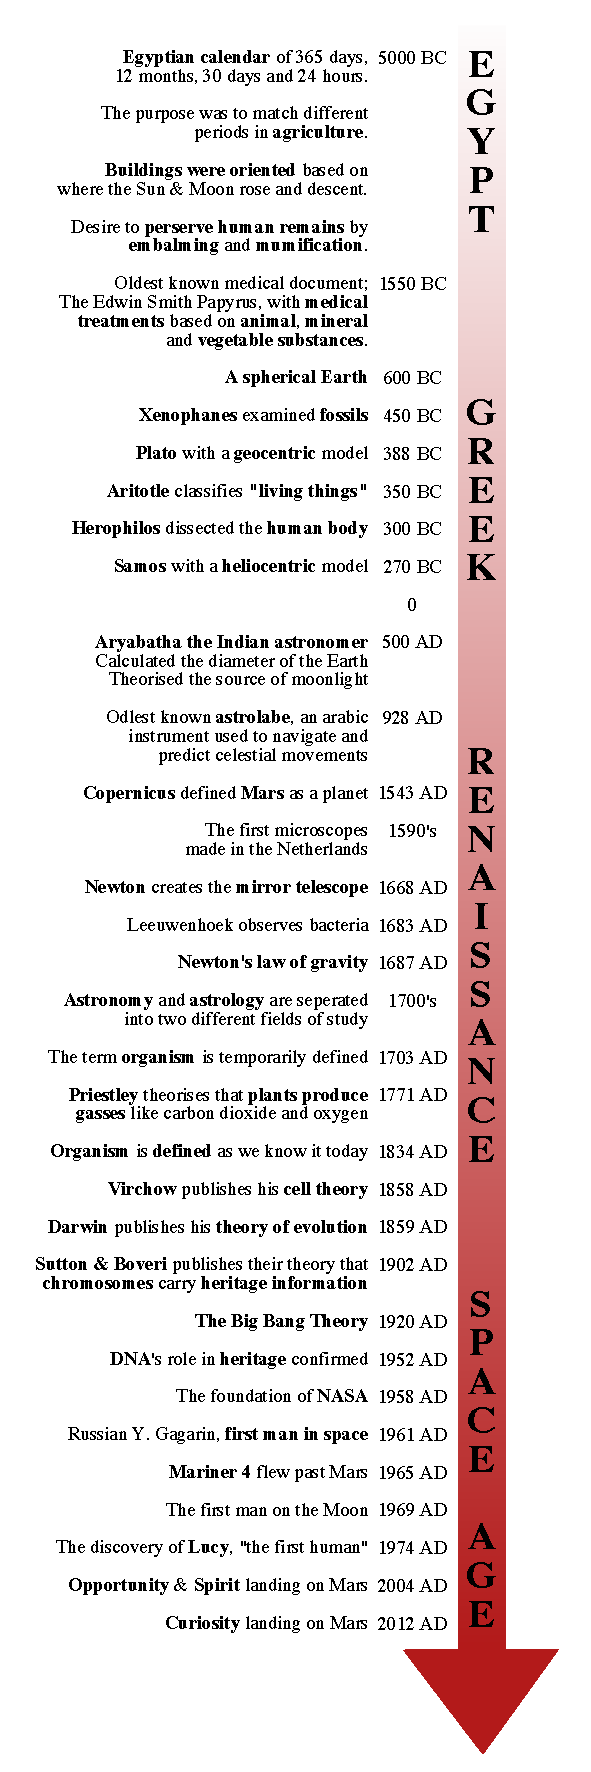
\includegraphics[width=0.475\textwidth]{timeline.pdf}
\end{center}

\subsection{Ancient Greeks, Arabs and Indians: The age of theories}
\initial{I}t is not until the Greek period, starting around 600 BC, that humanity tried to really understand and explain astronomy. 
To start with, they thought that Earth was flat, surrounded by water and that the stars were emerging from it.
Plato, followed by Ptolemy and Aristotle, were the pioneers of the geocentric model: the Sun, the Moon and the planets move in harmony around Earth, the center.

A hundred years later, another Greek, Samos, proposed the opposite theory called heliocentrism: the Sun is now the center of the Universe.
How fascinating to see how much they actually discovered at that time!  
Without tools such as the telescope, without communication within the community of scientists around the world, Greeks, Arabs and Indians still made great assumptions on how our universe worked. 
For example, the Indian astronomer, Aryabatha, not noly did he have some ideas about gravitation but also that the movement of planets around the Sun were elliptical and not circular.
He even understood that the light coming from the Moon was refracted sunlight, and not the Moon itself glowing in the dark sky.
One might wonder, how much we would know in the present time if ancient astronomers had the tools of communication we have today?
\cite{GreekAstro}
\cite{Aryabatha}

\subsection{European Renaissance: The age of reason and experimentation}
\initial{W}ith new technologies and the rediscoveries and translations of ancient Greek texts, the scientists of the renaissance period, were able to make very accurate calculations of the stars and planets.
Intellectuals in this period defined and proved the basic of astronomy as we know it today.  
Scientists such as Copernicus, Galileo and Kepler defined the heliocentric model to the world. 
It was definitely the age of reason and scientific truth. 
We can notice for example, that it is during that time that astronomy and astrology were separated into two different fields. 
Technologies and communications became more advanced and enabled physicists to search deeper and with more accuracy. 
In 1609, the Italian astronomer Galileo was one of the first people to point a telescope skyward. 
Although that telescope was far from perfected, Galileo was able to see that the Moon's surface was made of craters and mountains instead of being smooth as we thought.
As their view expanded dramatically by the telescope, astronomers were also able to discover many stars and to calculate stellar distances.
\cite{GalileoTelescope}

\subsection{Space Age: Not only studying Astronomy but also Exploring!}
\initial{I}n 1957, The Soviet Union launched Sputnik, the first spacecraft placed in orbit around Earth, marking the beginning of space exploration.
We are not only interested in studying, but also of exploring.
The space age represents an effort that is as scientific as it is political.
Indeed, this happened during the Cold War when the Soviet Union and the USA raced in different domains, including astronomy.

This space race focused particularly on discovery by humans and machines in the solar system and the development of technology.
Rockets were one of the most obvious forms of space age technology.
The creation of NASA, followed by the Apollo program was definitely highlights of the space age.
The most famous of the Apollo aircrafts was Apollo 11, carrying commander Neil Armstrong and his fellow astronauts Michael Collins and Edwin 'Buzz' Aldrin to the Moon.
On that mission, Armstrong and Aldrin were the first humans to land and walk on the Moon.
"That's one small step for a man, one giant leap for mankind."
\cite{SpaceAge}

\vspace{5mm}

\begin{tcolorbox}[colback=green!5,colframe=green!40!black,title=The wow! signal: Our first Extra-Terrestrial communication ? ]

On a night in 1977, Jerry Ehman, working for SETI (Search for Extra-Terrestrial Intelligence) took part in one of the world's biggest mysteries: The Wow! signal.

He was working on radio frequencies used as signals. The system is simple:\\

We measure intensity of radio frequencies. The intensity goes from 0 (the lowest) to 35 (the highest).  The intensity of the signal is normally between 0 and 2. But for 72 seconds he got an extraordinary signal: 6EQUJ5 from non-solar origin. A signal that was at its highest (the letter U) 30 times greater than the ordinary deep space noise! Amazed, Ehman wrote on the side: "Wow!", which simply became the name of the signal. But despite different theories and research on this signal, we still have no clue on what happened that night in 1977... \\

\textbf{What is 6EQUJ5?} \\

The intensity is measured between 0 and 35. Instead of just using numbers we changed 0 into a space and each numbers after 9 with the corresponding letter of the English alphabet. For example Q= 26 and U=30 

\end{multicols}

%------------------------------------------------

\section{Physics crash course}

\begin{multicols}{2}

Now that we have begun building our foundation of knowledge with history, we need to add some science basics. To fully understand life and how to define it, some \emph{biology} basics are required; how life works at the smallest levels, how it is built and rebuilt, and what the different components mean. To understand the science of the tools used to find this life, one has to be schooled in \emph{physics}, and how the field's analysis methods work. Physics also introduces us to entropy as a concept that can be used to define life. Let's begin there:

\subsection*{Entropy}
Imagine a room full of balls bouncing off the walls and each other.
Your image is probably a chaotic mess of balls traveling in all directions and speeds.
The order, or disorder, of the balls is what physicists call entropy.

Entropy is derived from thermodynamics, and it explains some of the most fundamental laws of our universe.

To understand what entropy really means, imagine all of the bouncing balls in your room being in the same corner at the same time.
This must be a very unlikely occurrence.
There are few ways to place all of the balls together in one corner, but lots of ways to spread them all around the room.
When all the balls are in the corner, the room has a low entropy.
If the balls are all over the place, the entropy is high.


The second law of thermodynamics says that the entropy in a closed system never decrease.
In other words; no matter what happens in a closed system, for example a room with no interaction with the outside world, there will be more and more chaos over time.
The system, or room, will eventually reach what we call a thermodynamic equilibrium.
If you want to keep the order in you room, you will need to supply it with energy.
That is partially why humans needs to eat.
Our cells use energy in chemical reactions, and we need to keep the entropy low in order for these chemical reactions to continue.
That is living beings has to be able to work against an increase in entropy, and also the reason this is one of the requirements we use to define life as we know it.

\subsection*{Spectroscopy, radiation and nuclear physics}








Spectroscopy is a method used in experimental physics to obtain information about a material.
In general one sends some kind of radiation towards the material, and then observes what happens afterwards.
Common radiation used in spectroscopy is photons, alpha, beta and gamma radiation.



\subsection*{Diffraction}





\end{multicols} \noindent\makebox[\linewidth]{\rule{\textwidth}{0.4pt}}

%------------------------------------------------

\section{Biology crash course}

\begin{multicols}{2}

\initial{N}ow that we are armed with a knowledge of the physics we need, we can move on to the biology. Here we are going to examine the most basic building blocks of life and the tools they use, and how they work together. This lays the foundation for an understanding of life at the microbial scale, which is the scale we expect to find life in our solar system.  Should we find it.

\subsection*{DNA}
\initial{T}he A in DNA stands for acid.
The rest stands for deoxyribonucleic, and describes the sugar structure around the acid. In the following section, the subparts of DNA and how they work together will be explained. 

The DNA molecule is the cornerstone of genetic determination; what defines you as you, and what describes the physical traits you will have.
It is the storage of the data that is you.
Each individual cell in your body - of which there are \emph{trillions} - contains 46 \emph{chromosomes}, which is the name for the coiled up DNA molecule.
Each DNA molecule has a special configuration of \emph{nucleotides} that determine what you will look like and how you will act.
There are enough miles of DNA wound up in each of us to make it \emph{to the Sun and back} 600 times!
That is a lot of tape to stick data on, and you see the manifestation of that variation in the flora and fauna of planet Earth.
There are a lot of different options available to genetics, and we will look at some of them and how varied they are later in the article.

\subsection*{Nucleobases and nucleotides}
\initial{N}ucleotides are worth knowing a little about, given how important they are to you and your uniqueness.
Biology considers four molecules to be the building blocks of everything else: carbohydrates, lipids (fats), proteins and nucleic acid.
We are interested in the acid - this is the defining element of DNA, which in turn is the defining element of us.
In the acid of DNA we find \emph{nucleobases}, which are the smaller jigsaw pieces of the bigger jigsaw puzzle that is DNA.
There are four kinds of nucleobases in DNA - you have most likely seen their abbreviations before; A for adenine, C for cytosine, G for guanine and T for thymine.
These four nucleobases bind to sugar and a phosphate group in various patterns to form a \emph{nucleotide}.
The order of the nucleotides in the DNA helix is what gives you brown hair, or good muscles for climbing, or an acute sense for pattern recognition, even how wet or dry your earwax is.
It is all determined by little sequences of acids in the core of your many cells.

The DNA helix is given structure by the sugar.
The sugar is what the nucleotides attach to, which can have some different configurations, and the little nucleotide units connected to sugar are again connected to each other by the phosphate.
In summary, the nucleobases with their many different configurations form the rungs of the DNA ladder.
The sugar and the phosphate are the rails that binds the rungs together.

\subsection*{Enzymes}
\initial{I}t is worth mentioning enzymes for how important they are to your body.
Enzymes are, in short, your body's power tools.
They are catalysts that speed up chemical reactions.
Pepsin, for example, is the enzyme that lives in your stomach acid and digests your food.
In your mouth you have amalyse, which breaks down starch.
Each little enzyme has an "active site" - where the power tools are put to use - that allows the enzyme to either break a molecule into parts, or reversely, collect smaller molecules into a newer, lager compounds.
These enzymes make our world go round, and since they can put on different hats and work different areas, we have comparatively few of them.
Enzymes are key in cell division, which is how life multiplies. 

\subsection*{Cell division and copying}
\initial{I}n short, the way we go from a few cells to many cells to human being, is by splitting the DNA that defines us and subsequently copying that DNA.
This is where the enzymes come in handy, as they can split the DNA strand.
The enzyme responsible for splitting it up is called the helicase.
It moves down the rungs of the ladder and neatly breaks up the DNA strand, and two new and distinct single strands are formed.
Each need to be complemented with the correct nucleobase to complete the same pattern it had before.
Now, without getting too hardcore on the details, the DNA helix is split into two different strands: the leading strand and the lagging strand.
What seperates the two is how the nucleotides are tied to the sugar molecule - worth looking up if you want more details on the complexity of the DNA molecule.
For now, we will look only at what happens during cell division.
The leading strand has it easiest.
After the helicase enzyme has made its cutting way through, another enzyme called an RNA primer moves on down the line after it.
It has a sniff around about what kind of nucleobases are hanging in the breeze, and makes a few sample connections, leaving a blueprint.
After it is done, the DNA primer hands the rest of the factory work off to another enzyme called DNA polymerase.
The polymerase lumbers on down the entire strand after that, reading the blueprints from the primase, and builds the corresponding nucleobases where they are needed. 
Things are bit more chaotic on the lagging strand.
Here, the order of the nucleobases is not as easily readable.
The RNA primase, the blueprints boss of the DNA split, has to rush back and forth all over the strand to write different blueprints.
The DNA polymerase follows after the primase, huffing and puffing, and builds small subsections of the strand until construction is complete.
The final coat of paint is called DNA ligase, which solidifies the structure of the new-born DNA molecule.
Et voilà, we have the miracle of reproduction at a cellular level.
This, however, is also where things can go wrong.
Mistakes are made - once every 10th billion nucleotide or so - the construction team messes up and builds a window where a wall should have been, or a tower where a roof should have been.
This is genetic mutation.
Mutation is the reason why we have centipedes and monkeys.



\end{multicols} \noindent\makebox[\linewidth]{\rule{\textwidth}{0.4pt}}

%------------------------------------------------

\section{Origins of life}

\begin{multicols}{2}

\initial{S}omehow, someway, we came from something and became this.
The world around us and all the living things in it were not always so, and the amount of time that has passed since our planet was the new kid on the block is so astoundingly massive that we cannot really conceive it.
This is not our fault - the biology of our particular form of life simply is not designed to mentally cross such vast gulfs of time.
Knowing how it all began becomes quite difficult, and the only thing we can say for certain is that we do not know for certain how it started.

\initial{W}e have made theories about this for a long time, and for most of that time those theories were founded in theology.
If you went back in time and asked an Assyrian, she would claim that life originated from the great god-emperor Ashur.
If you go forward in time a bit and ask the Greeks, and they will point you to the stars and the fathers of their gods, the Titans.
Go forward a bit more and you will hear christians tell you that life was formed out of clay by Yahweh.
(Unless you are a woman, in which case you were made out of a man’s rib.
The sparerib theory?) 

\begin{center}
	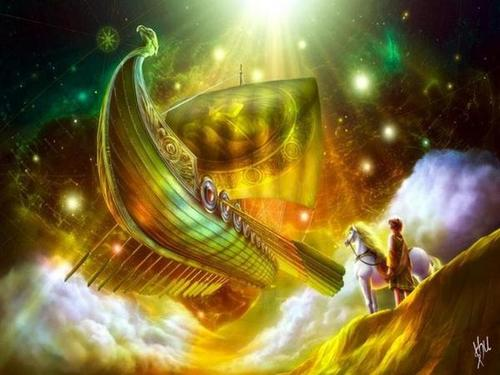
\includegraphics[width=0.45\textwidth]{magicship.jpg}
\end{center}

\initial{T}he painting of the magic ship might not be that accurate, but the theological theories are pretty cool.
(This particular image was painted by Kagaya Tomonori.)
We have gotten a bit more methodical since then, and we know a bit more about the specifics of life, so we have constructed some better models.
Modern, scientific theories have limited it to a narrow method involving RNA and interactions between chemical compounds in pools of primordial liquids.
We know the basic ingredients to the recipe, but exactly how to cook is just theorized.
We can line up all these ingredients in vials in a lab, walk down the line past them; all we need is water, specific monomers and minerals, and energy.
Take a moment to consider how bizarre it is that given pressure and time, the contents of the vials have turned into beings capable of painting the Sistine chapel and landing robots on comets.
From oozing, primordial goo to beings capable of producing masterworks of art and technology.

\initial{T}here are three different theories worth mentioning, and it also worth underlining that these are not assertions of truth.
The three theories are all pretty tasty; respectively the soup, pizza and sandwich theories.
Let us dig in!

\subsection{Soup}
\initial{T}he soup theory is the first and most basic modern model of the origin of life on earth, and was formulated by the soviet biologist Alexander Oparin way back in 1924.
It postulates \cite{shapiro} that (billions of years ago mind you) in the time when the planet was a toddler, the atmosphere was weaker and the elements on earth were more directly exposed to energy waves from space.
This energy worked as a catalyst on simple chemical compounds - called monomers - which met for parties in the pools and eventually fused to create more complex compounds.
With enough partying, these monomers turned into RNA, and the RNA eventually gave us photosynthesis and respiration - the two key ways lifeforms harvest energy.
What we do not know is how this fusion happened, and we do not know how the RNA led to DNA. 
That is it for starters, onwards to the main course, the pizza theory.

\subsection{Pizza}
\initial{W}hat separates the pizza from the soup is the spatial dimension, which is useful ith regards to our laws on life and entropy\ref{entropylol}.
It is very similar to the soup, but instead of large primordial pools, the pizza postulates that it is more likely that life originated in shallow basins of water near the surface \cite{Exoboken}. 
This gives two clear advantages over the soup: access to flat surfaces of rocks containing tasty minerals, and a closer proximity to the energy waves of the sun.
This trifecta is a bit more proximate and powerful when in a shallow, "two-dimensional" space, as the Sun’s rays can hit both the monomers and the minerals and catalyze the partying between them all even more.
There is a problem with this theory as well.
It does not explain how the earliest monomers got the right amount of water to form stable polymers.
Since the pizza theory has some holes, a third theory has been presented, and like a sandwich, it involves layers.
Enter the sandwich.

\subsection{Sandwich}
\initial{T}his theory is again similar to the others, but the difference here is the delivery mechanism of the catalyzing energy \cite{szosa}.
This theory postulates that life may have begun in the tiny spaces between layers of the mineral mica.
These spaces precisely correspond to the size of the earliest compounds (a single nanometer).
The layers of mica are so atomically flat that even the tiny DNA molecules show up as ridges on the surface when examined under a microscope.
Furthermore, the electrical charge of RNA and the earliest lipids (which are fats) matches the electrical charge of mica.
Both RNA and protein can be, and have been formed in laboratory conditions.
Both the water missing from the pizza and the energy missing from the soup are applied through lapping waves, which contain both water (obviously) and mechanical energy.

We have now looked at modern theories for how life originated on our planet, and how it could originate on other planets given similar conditions. What kind of forms does it take here, on our planet?

\end{multicols} \noindent\makebox[\linewidth]{\rule{\textwidth}{0.4pt}}

%------------------------------------------------

\section{Defining life}

\begin{multicols}{2}

\initial{T}he seemingly trivial terms life and being alive have meanings most of us think we understand.
Surprisingly, an exact definition of life does not exist.
Instead, there has been established a list of criteria we think need to be fulfilled in order to be called life.
Such a list is given in Kjetill Østgaards \textit{Exobiologi - A hitch-hikers's guide to alien life} \cite{Exoboken} and those criteria are the basis for this section.
Considered separately, and possibly also as a whole, these criteria does not exclude examples of phenomena and machines we would not consider to be alive.
The debate concerning what life really includes is therefore open to all kinds of meta discussions and creative thinking.

\subsection{Growth}
\initial{T}he first typical criterion defines life as something that grows.
Growth is here referring to physical growth as part of a life sycle, and not personal or mental growth.
For mammals, the growth cycle starts at birth as an infant, then proceeds through the stages of youth and adulthood before ending up as an elderly individual until death.
Insects proceed through stages called egg, larvae and pupae before reaching the fully developed form of adulthood.
Both these examples are undoubtedly forms of life as we know it, but examples of inorganic phenomena subject to growth are also common.
The classical example is crystal growth describing the formation of strictly organized solid lattices.
Another example is the surface of Earth itself.
In plate tectonic theory \cite{tectonic}, the cycle of the Earth's crust can be explained by colliding and parting plates.
In a boundary zone where two plates move apart from each other, magma from inner Earth will erupt from the fissure as lava and form new crust.
In a collision zone a subduction will occur if one plate is forced underneath another, becoming part of the inner mantle.
This growth cycle of course spans over a much longer timescale than that of a mammal, but so does a mammals cycle compared to most insects.
Obviously this criterion alone does not describe life as we know it.

\subsection{Metabolism}
\initial{N}ext criterion will exclude both the crust and crystals as life forms.
It claims that a living organism must be able to support chemical reactions called metabolism.
This means that life must be able to generate new, complex molecules in a process called anabolism and to break down complex molecules into simpler ones in a process called catabolism.
In mammals, the result from anabolism is physical growth and muscle development from nutrients retrieved in the catabolism of food.
On the contrary, a chemical reactor will be able to maintain both destructive and productive reactions without actually being alive.

\subsection{Reproduction}
\initial{P}erhaps the most commonly known criterion is that life needs the ability to reproduce itself.
Humans and animals produce offspring, which contains a different set of genes than their parents.
This process called sexual reproduction requires the fusion of two sex cells \cite{reprod}.
Less complex forms of life can reproduce by simply dividing into two as some bacteria, by pollination as with most plants or by spore formation as with fungi and protozoa.
Such asexual reproductive processes will result in an offspring containing identical genetic information as the origin.
A virus - the odd one out - is not able to reproduce by itself and is dependent on its host cell in order to survive.
Thus a lot of people do not consider viruses to be life.
An even more extreme example is the offspring of a donkey and a horse.
The mule is a sterile animal, even so, most people would recognize a mule as a living organism regardless of this fact. 
Not to mention animals and humans that are born sterile or surgically made sterile.
Organic life does not have the monopoly on reproduction. Documents are easily reproduced in a copy machine, and biotechnologists have succeeded reproducing DNA in advanced PCR-machines.
The science of cloning is also widely developed and has succeeded in duplicating a living organism without the methods of traditional reproduction.
In other words, the criterion of reproduction would exclude a sterile cat as being alive, but may include inorganic phenomena that are possible to reproduce by itself or others.

\subsection{Evolution}
\initial{I}n 1859, Charles Darwin introduced the well known theory of evolution in a book called \emph{On the Origin of Species} \cite{Darwin}.
The basic idea of biological evolution is that all life on Earth shares a common ancestor!
As a result, all species roaming the Earth today are very distant cousins.
This means that all living species have a placement, according to their inherited characteristics, on a family tree.
A family tree is a representation of the evolutionary relationship among species.
This theory states that life has evolved based on a principle called \emph{survival of the fittest}.
This has resulted in the survival of the species, and the genes of the species, which were best adapted to their environment. 

On a computer, such an algorithm can easily be implemented.
The best known example is John Conway's \emph{Game of Life} \cite{Conway} which illustrates natural selection by defining four simple rules determining if a cell will live, die and/or reproduce.
The rules determining the future of one cell are all concerned with its neighbours and environment:
\begin{enumerate}
\item Any live cell with fewer than two live neighbours dies, as if caused by underpopulation.
\item Any live cell with two or three live neighbours lives on to the next generation.
\item Any live cell with more than three live neighbours dies, as if by overcrowding.
\item Any dead cell with exactly three live neighbours becomes a live cell, as if by reproduction.
\end{enumerate}
Applying these rules to all cells in a grid will lead to changes in the total amount of cells and their position for the next generation.
After applying the rules for a number of generations, the grid will look very different, but is in fact a direct outcome of the initial condition.
Evolution has taken place! 
There is now also a solid foundation for man-made evolution, the so called \emph{augmented human being}, which many of us already are.
The invention of eyeglasses is a trick on evolution - those with poor eyesight haven't evolved their way out of the problem, but have built themselves out of it instead.
Augmented humans are taking off in the coming century - \emph{biohackers} have already injected their eyes with chemicals from deep-sea fish to gain temporary nightvision\cite{biohack}, exoskeletons are being made that can help the paralyzed walk, and there are blueprints for nanorobots that can simulate blood cells and do what they do far more efficiently\cite{nanoblood}. 

\subsection{Motion}
\initial{T}he last criterion that is being considered is the phenomenon of motion.
All living organisms should be able to move and often as a response to different stimuli.
Mammals, fish and birds have either legs, fins or wings making them capable of moving their entire body.
The motion can be in an attempt to escape as a response to a threat, in chase for food or water in order to survive or simply just in order to transport itself somewhere.
In almost every activity a human can perform, a specific motion is required.
Plants are not able to move their entire body, but in order to efficiently trap sunlight, plants can turn their leaves towards the Sun.
A lot of non-living machines or vehicles are also able to move, and more and more can move on autopilot.
There also exist solar panels that can trace the Sun much like a plant, and robots that can walk and perform tasks much like a human.
Whereas some living things, like coral reefs, do not move at all.
If motion was the only criterion to be fulfilled, life would include a much wider spectrum of phenomena.
Expressions like \emph{"This storm seems to come to life with its motion, power and shape"} and \emph{"Tales come to life in the forest"} would all of a sudden have a literal interpretation. 


The past section presented and reflected on the criteria creating a definition of life.
Hopefully it became evident that a simple, straight forward definition is hard to formulate considering that the term \textit{life} must include, yet also, exclude so many phenomena.
Although there are tons of non-living examples on each of the presented criteria, the combination of properties concerning growth, metabolism, reproduction, evolution and motion are a valid basis for living creatures.
That means, of course, living creatures as we know them.
If these criteria also apply to extra-terrestrial life, only the future can answer.
Perhaps completely new lifeforms, extremely different from all earthly life, will be discovered.
With that in mind, it is an advantage that the definition of life is not carved in stone. 


While we struggle with finding a precise definition for life, we know a lot about what makes the life we have tick. A lot of the hullaballoo on Mars has been about finding \emph{water}, which is the lowest common denominator for all life as we know it. 

\end{multicols}

\noindent\makebox[\linewidth]{\rule{\textwidth}{0.4pt}}

\section{Life forms on Earth}

\begin{multicols}{2}

\subsection*{Life forms on Earth}

It is easy to forget the many shapes and styles life on our little planet takes. On a stroll along the seaside, you will walk past lifeforms so strange and different from you that when given deeper thought, they seem positively alien.
Consider the grass, which consumes sunlight to live and grow. Consider the life of the oyster, buried under the sand of the shoreline you walk past.
Consider the life of the seaweed, drifting at the surface, and how bizarre that existence seems when compared to your own.
We get used to it, since we see it all the time, but to give it thought and time to study can give a profound impression of the incredulity of life on Earth.

So, what kind of lifeforms exist on Earth?
Is it just one long list of different species, or are there ways to divide it on a more fundamental basis?
The second option is fortunately the right one.
When comparing life on a molecular level it can be divided into three primary groups (or domains): bacteria, archaebacterial and eukaryotes \cite{Eukaryotes}.
Bacteria and archaebacterial go under the collective term prokaryotes.
The difference between eukaryotes and prokaryotes is considered the most important distinction among living organisms \cite{Procaryotes}.

Prokaryotes are single-celled organisms living in clusters or colonies while eukaryotes can be both unicellular and multicellular.
Prokaryotes reproduce asexually meaning it clones itself, which we humans can't do quite yet, while most eukaryotes reproduce by mixing the parents genome \cite{ProcaEuka}.

An easy way to consider this is that prokaryotes are like bacteria (very small and 'simple' life forms) and eukaryotes is the things that is more familiar for us, like plants, mushrooms, animals as well as you and me.
While complexity seperates us, we all come from the same origins, which in and of itself is an astounding thought.

The theory is that the common universal ancestor of all life was a prokaryotic cell and that the eukaryotes were created by prokaryotes fusing \cite{ProcaEuka}.
This is analogous to us, as human beings. You think of yourself as just yourself, right? The being behind the eyes, looking out, observing, thinking, interacting.
It's just you.
'˜Just you', as complex as you are with your ability to laugh, love and create, is a living form consisting of trillions of other lifeforms, dancing together in a complicated dance every second of every day of your life.
All the cells in your body, all the external bacteria such as the flora in your gut that helps you digest food, all the enzymes and neurons and proteins, all can be considered their own living entities.
They all work together to make you \textit{you}, and all of this happens without your input.
The coordination between these lifeforms at the lowest level is natural and not planned - the cells in your hand don't meet with the cells in your lung at the pub and ask, 'hey, what do you do for a living?'
They aren't even aware of each others' existence.

This leads elegantly into an emerging theory on our planet itself, the Gaia theory \cite{Lovelock}.
Now this is a theory, but it's an interesting one, and it's worth noting, especially with what we now know of the unwitting coordination of the cells in our body.
Gaia theory, originally concocted by a chemist named James Lovelock in the 60's, is about how the very planet we live on can be, just as we are, a single organism consisting of trillions of lifeforms working together, unwittingly.
Could it be that we are just cells in the body of the planet Earth?
Are we zooming around the sun in a single organic spaceship?
Could we, in the future, as our space travel talents grow, encounter living planets as singular entities?

\end{multicols} \noindent\makebox[\linewidth]{\rule{\textwidth}{0.4pt}}

%------------------------------------------------

\section{Water}

\begin{multicols}{2}

\noindent
\initial{P}lanet Earth is often called the blue planet due to the dominant blue areas visible when viewing Earth from space.
The blue areas are our vast oceans covering more than 70\% \cite{WikiEarth} of the surface.
These oceans contain and support a broad spectrum of life, and are also a great influence on the Earth's climate and weather.
All species on Earth, eukaryotes and procaryotes alike, are dependent on water in order to survive.
A human can only survive for 5 days without water \cite{SurviveWater}, and even extremophiles called xerophiles, dry loving bacteria, need a tiny amount of water in order to function.
In other words, water is essential to life as we know it and therefore extremely interesting. 

\subsection{Chemical properties}
A single water molecule consists of three atoms: one oxygen atom and two hydrogen atoms.
The two hydrogen atoms are bonded covalently to the oxygen atom.
Due to two lone electron pairs on the oxygen, with their electrical pull, the overall structure of the is bent.
The lone pairs are not shared between the atoms.
Furthermore, the oxygen atom is much more electronegative than the hydrogen atoms, creating a dipole moment in the molecule.
This means that the oxygen will contain a slight, but significant negative charge while the two hydrogen atoms appear as slightly positive.
This creates the basis for the formation of an intricate network of hydrogen bonds as we know that positive and negative charges attract one another.  

So what makes water so unique?
First of all, the formation of hydrogen bonds gives water a high evaporation entalphy and therefore a large evaporation temperature.
To transform water from its liquid phase to vapor, energy must be applied bringing water to a temperature of 100\degree C.
On the other end of the scale, water will freeze at 0\degree C transforming to ice, which brings us to the second uniqueness of water.
In most cases, a solid phase will be denser than a liquid phase.
Thus the solid phase would sink to the bottom of the liquid phase. \cite{SolidWater}.
Polar bears floating on ice flakes in the Arctic are evidence that ice is not heavier than water.
This phenomenon has had a greater importance than just serving as a fleet for polar bears.
Without this property, ice would have sunk to the bottom in repeated cycles until there was no more liquid water during the cold periods in the history of Earth.
To sum up, due to chemical and physical properties, water remains liquid over a uniquely broad range of temperature.

However, the temperature is not the only thing that decides phase states in matter.
Pressure is equally important.
Therefore one can boil water at 70\degree C at the top Mount Everest (making it hard to boil an egg), while you need to heat it to 100\degree C at sea level \cite{WaterEverest}.
The diagram shows how this relationship between temperature and pressure affects the states of water.

\end{multicols}

\begin{center}
	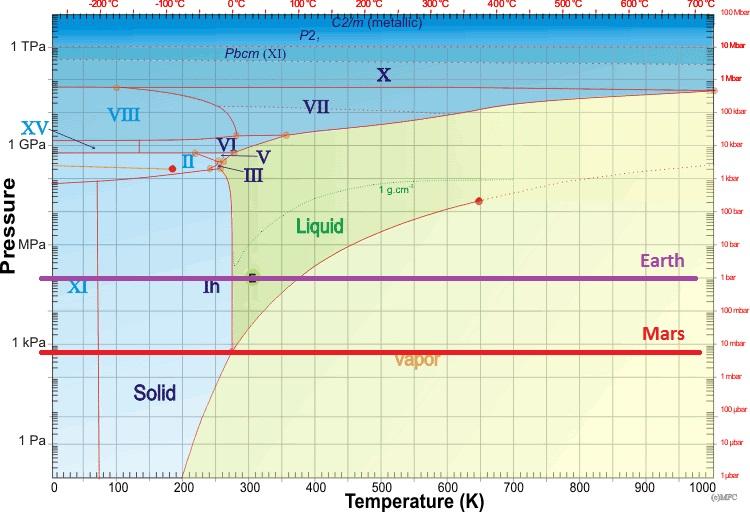
\includegraphics[width=0.9\textwidth]{water_phase_diagram_2_merka.jpg}
	% kilde: http://www1.lsbu.ac.uk/water/water_phase_diagram.html
\end{center}

\begin{multicols}{2}

Notice that although water can appear at Earth's 1 atm, which is about 101 kPa \cite{AtmEarth}, the pressure of 0,006 atm at the Martian surface \cite{AtmMars} does not allow water to be liquid.
An attempt to melt ice on Mars will result in sublimation.
The mean temperature on Earth is 15\degree C \cite{WikiEarth}.
This along with the pressure of 1 atm it makes Earth a perfect place for liquid water. 
So far, we have established that we have a lot of water on Earth, and it occurs mostly in its liquid form.
The question remaining is: what is so important with liquid water?

Liquid water has functions as both a solvent and a transport medium.
Both organic and inorganic compounds can be dissolved in water, making it a vital part of metabolism.
The blood stream is an essential transport network delivering oxygen and nutrients in our body.
Human blood plasma, the liquid part of the blood, consists of 92\% water \cite{Blood}.
On Earth, we have yet to find an organism completely independent of water. 
In fact, in all three theories concerning the origin of life, water was given a leading role as a solution bringing the organic molecules together.
As we want to find life, it seems appropriate to base our search on water.
NASAs guiding policy reflects this: \textit{Follow the water} \cite{NASAwater}. 
Water is not a rare molecule in space, in fact oxygen and hydrogen are some of the most abundant atoms in the universe.
The only problem is that the water in space most often is in the solid form of ice, and in rare occasions in form of gas.
There have been discoveries of water on Mars. 
Both poles have ice caps containing solid water \cite{MARSwater}.
Unfortunately, solid water does not have the same solvating and lubricating properties as liquid water, and will therefore not support molecular processes essential for life.
However, dry channels and craters probably formed by erosion suggest that liquid water (or some other liquid) once was present on Mars.
The best signs of life in space is therefore the discoveries of molecules we know can only be formed in contact with water.
For example, in 2002, Mars 2001 Odyssey, which is orbitting Mars, found the spectral signature of hematite, a molecule formed in water.
This mineral was later discovered by Opportunity, one of the two twin rovers exploring Mars from 2004 to 2010.
Furthermore, in 2005, Spirit, the other twin, found high concentrations of carbonate which originates in wet, near-neutral conditions. 
Carbonate actually dissolves in acid, which means that the water on this area could not have been acidic.
The rover roaming the surface of Mars today, named Curiosity, continues seeking for evidence of water. 
Where there is liquid water, there might be alien life.

\end{multicols} \noindent\makebox[\linewidth]{\rule{\textwidth}{0.4pt}}

%\begin{multicols}{2}

%\end{multicols} \noindent\makebox[\linewidth]{\rule{\textwidth}{0.4pt}}

%------------------------------------------------

%\section{Entry, decent and landing (EDL)}

%\begin{multicols}{2}

%\section*{Entry, decent and landing (EDL)}
\initial{A}fter a successfully launch from Earth at Space Launch Complex 41 on Cape Canaveral Air Force Station in Florida at 10:02 a.m. EST, Nov. 26, 2011 a 563 270 400 km travel awaited for curiosity \cite{MissionTimeline} \cite{CNNCuriosity}.
When reaching the Martian atmosphere the Entry, descent and landing phase (EDL) began, a spectacle popularly known as seven minutes of terror \cite{CNNCuriosity}.
Because of Curiosity's large weight and size, it could not utilize the landing procedures used for earlier rovers.
In fact, this landing method has never been tried before.
It is as unique as it is complicated, thus the name seven minutes of terror (referring to the time it takes Curiosity to land on the surface after touching the Martian atmosphere) [8].

The EDL sequence breaks down into four parts; guided entry, parachute descent, powered descent and the sky crane \cite{NASALanding}.


\begin{center}
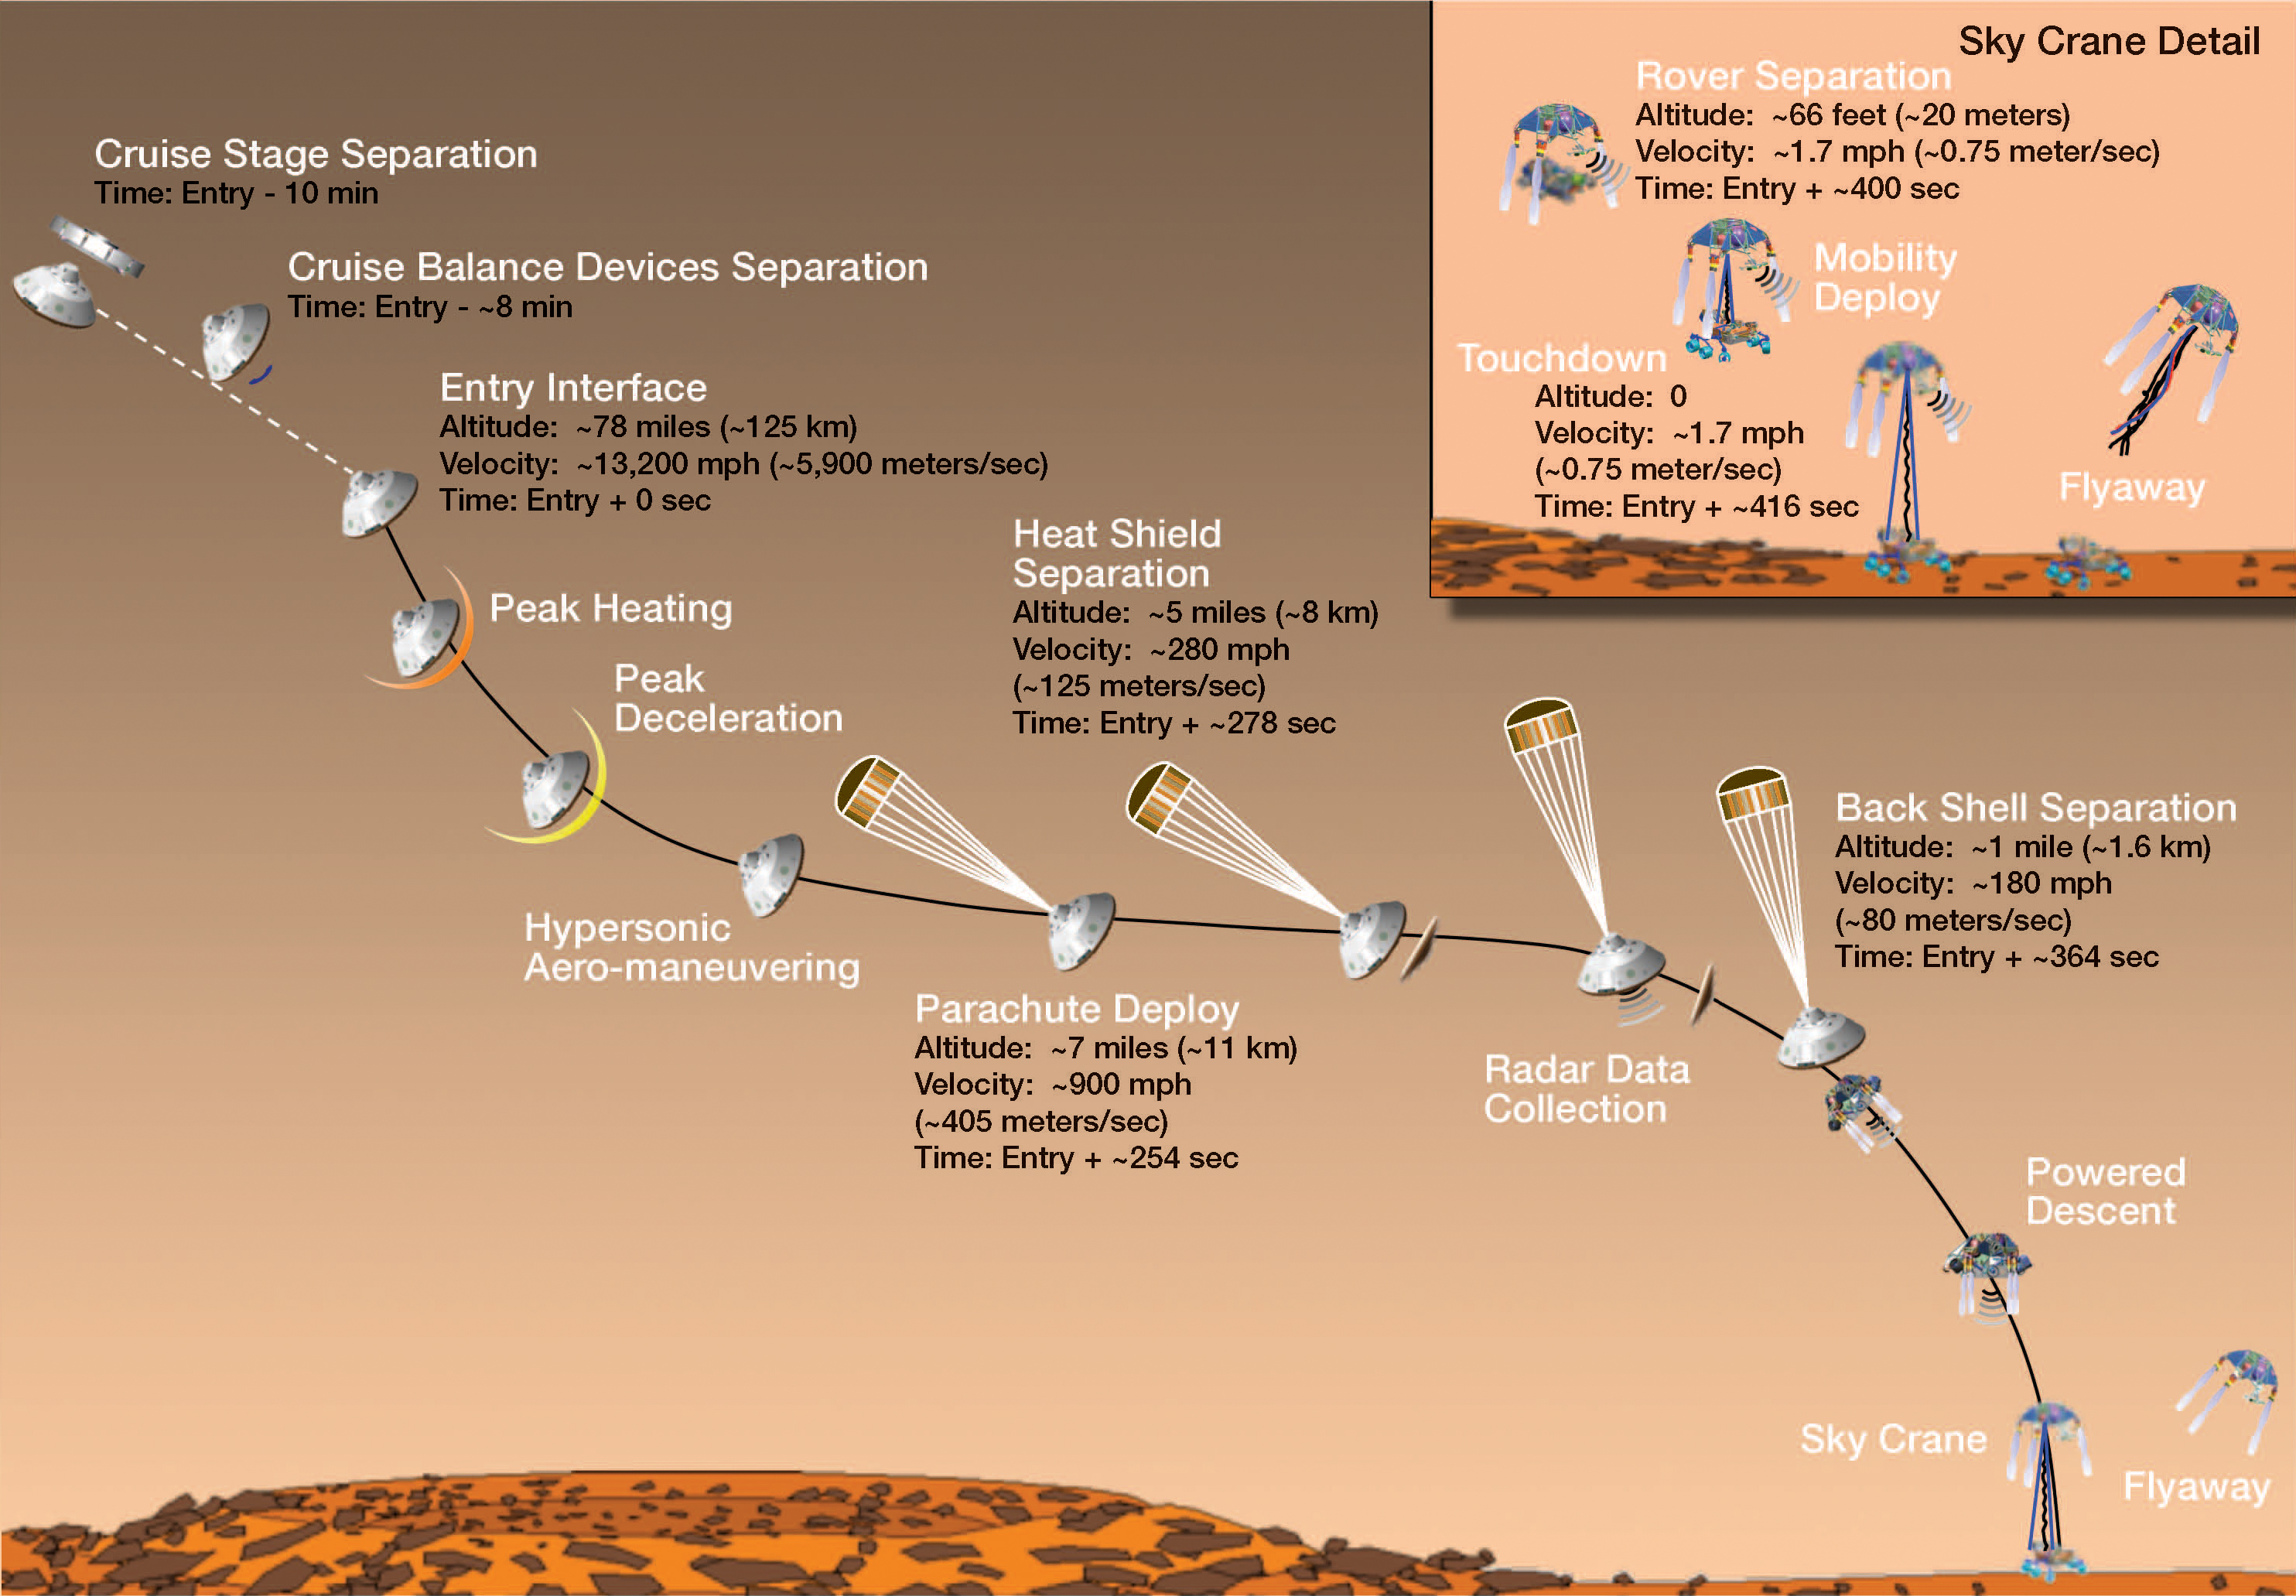
\includegraphics[width=0.5\textwidth]{Curiosity_landing.jpg}
\label{fig:Curiosity_landing}
\end{center}


\subsection*{Guided entry}
\initial{10} minutes before reaching the atmosphere the cruising stage is detached and burns up.
With a velocity of 21 240 km/h it slams into the Martian atmosphere at an altitude of 125 km [4]. Creating so much aerodynamic drag the heat shield reach a temperature of 2100?C glowing white hot \cite{NASALanding} [5]. Being the first spacecraft to use precision landing techniques on Mars the name ?guided entry? refers to its ability to adjust it course during this first stage. The course adjustments will be controlled by four sets of two Reaction Control System (RCS) thrusters. Each pair capable of generation about 500 N (50 kg) of thrust [7]. Where the Mars Exploration Rovers could have landed anywhere within their respective 150 by 20 kilometers landing ellipses, Curiosity landed within a 20 kilometer ellipse \cite{NASALanding}.
The Martian atmosphere is extremely difficult to slow down in because it has just enough atmosphere that you have to deal with it (or else your spacecraft is destroyed), but still too little to get the job done [5]. The heat shield only manages to slow the spacecraft to a speed of 1620 km/h in which time the deceleration has created a maximum force equal to 15 G?s \cite{NASALanding} [7]. This is still way too fast for a safe landing and brings us to the next step.

Parachute descent
At an altitude of 11 km, the largest and strongest supersonic parachute ever constructed for an extraterrestrial flight deploys \cite{NASALanding} [6]. Deploying at such speeds creates a neck snapping 9 G?s [5]. The parachute with a diameter of nearly 16 m has 80 suspension lines measuring more than 50 m in length and would be capable of generating 24 500 kg of drag force [6]. About 8 km over the surface the heat shield poops of giving a clear view for the radar. The radar calculates altitude and speed determining when to initiate the next phase \cite{NASALanding}.
The parachute will not be able to slow the spacecraft to a speed lower than about 280 km/h. This is still way too fast for a landing. Only one solution; separate the rover from the backshell and parachute \cite{NASALanding}.

Powered descent
The descent stage (includes the rover) now in free fall fires eight Aerojet?s variable thrust mono propellant hydrazine rocket thrusters and doing a divert maneuver to avoid colliding with the backshell and parachute \cite{NASALanding} [7]. Each of these rocket thrusters (called Mars Lander Engines or MLEs) are capable of producing 320 kg of lift [7]. The MLEs will slow the spacecraft to a velocity of 14.5 km/h while adjusting its position for the final stage. 

Sky crane
At an altitude of 27 m, the rover is detached from the descent stage and slowly lowered to the ground. While three nylon cords (communications between the rover and the descent stage is ensured by an umbilical line) lower the rover, the descent speed is reduced to 2.7 km/h. At 7.5 m, the cords are fully extended and the descent speed is kept constant at 2.7 km/h until the rover finally touches down \cite{NASALanding} [7]. The descent stages continues it decent velocity while the rover use 2 seconds to confirm full weight on all wheels. The cords and umbilical line pyrotechnically detaches from Curiosity and the descent stages assume command of itself. Tilting 45-degrees, it performs a flyaway-maneuver crash-landing at least 150 m away [7]. 
Despite everything that could have gone wrong the rover landed unharmed on the surface of Mars at 10:32 p.m. PDT on Aug. 5 2012 \cite{NASALanding}.


References


[4]	http://www.startalkradio.net/wp-content/uploads/2012/08/667372main\_MSL-EDL-rev-2900.jpg
[5]	https://www.youtube.com/watch?v=h2I8AoB1xgU
[6]	http://mars.jpl.nasa.gov/msl/news/index.cfm?fuseaction=shownews\&newsid=90
[7]	http://www.nasaspaceflight.com/2012/08/msl-curiosity-historic-martian-landing-at-gale-crater/
[8]	http://lightyears.blogs.cnn.com/2012/08/03/8058/

%------------------------------------------------

%\end{multicols} \noindent\makebox[\linewidth]{\rule{\textwidth}{0.4pt}}

%------------------------------------------------

\section{Curiosity}

\begin{multicols}{2}

\initial{T}ruth be told, water has already been fond on Mars.
Both poles have ice caps containing solid water \cite{MARSwater}.
Unfortunately, solid water does not have the same solvating and lubricating properties as liquid water, and will therefore not support molecular processes essential for life.
However, dry channels and craters probably formed by erosion suggest that liquid water (or some other liquid) once was present on Mars.

\begin{center}
	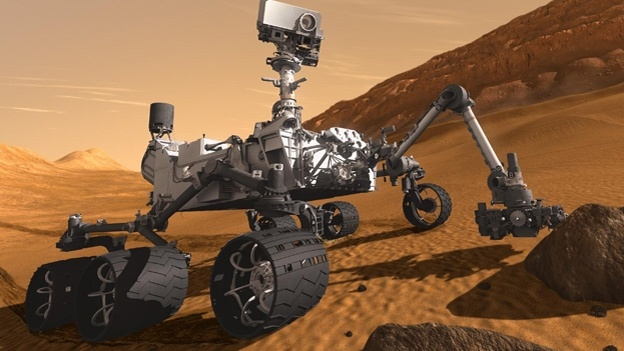
\includegraphics[width=0.45\textwidth]{Curiosity.jpg}
	NASAs Mars rover.
\end{center}

The best signs of life in space is therefore the discoveries of molecules we know can only be formed in contact with water.
For example, in 2002, Mars 2001 Odyssey, which is orbitting Mars, found the spectral signature of hematite, a molecule formed in water.
This mineral was later discovered by Opportunity, one of the two twin rovers exploring Mars from 2004 to 2010.
Furthermore, in 2005, Spirit, the other twin, found high concentrations of carbonate which originates in wet, near-neutral conditions. 
Carbonate actually dissolves in acid, which means that the water on this area could not have been acidic.
Hematite and carbonate are not the only minerals Curiosity is treasure hunting for.
In general, the rover uses its incredible instruments to study many different properties of the Martian surface.

\end{multicols}

\begin{tcolorbox}[colback=red!5,colframe=DarkRed!40!black,title=Curiosity: 10 facts about the rover]

\textbf{Purpose:} To investigate the climate and geology on Mars, and to find evidences for the presence of water.

\textbf{Travel:} From November 26th 2011 at Cape Canaveral Air Force to 6th August 2012 at the Gale Crater.

\textbf{Mission duration:} One Martian year, that is 98 weeks.

\textbf{Mass/size:} The mass is 900kg. The dimensions are 3m x 2,8m x 2,1m, about the size of a car.

\textbf{Movement:} The rover can travel by an average of 30m per hour.

\textbf{Instruments:} It has 17 cameras, most of them are used to drive and navigate.

\textbf{Energy source:} The onboard nuclear power plant carries plutonium-238. From the material's decay it can produce 125W of electricity.

\textbf{Computers:} The two identical computers are specially built to tolerate the radiation that occur on Mars. They have only 256MB of RAM and 2GB of flash memory each.

\textbf{Communication:} The rover uses its three antennas to communicate in the UHF band. Direct communication to the Earth takes about 7 minutes. The rover can also communicate via Mars satellites.

\textbf{Cost:} The overall cost was 2,5 billion USD, where 1,8 billion of it was used in context of freighting the rover to Mars.

\end{tcolorbox}

\pagebreak

\section{How does Curiosity search for water?}

\begin{multicols}{2}

\initial{A}s explained earlier, finding water on Mars is not the hard part.
Liquid water, on the other hand, is a whole other story.
The rover has a wide array of apparatuses ready to help the crew sitting on Earth with the biological treasure hunt.
Many of these are cameras used for driving and navigating.
Others are used to gather information.
We will focus on some them:

\begin{itemize}
\item Chemistry \& Camera
\item Chemistry \& Mineralogy
\item Alpha Particle X-ray Spectrometer
\item Dynamic Albedo of Neutrons
\item Radiation Assessment Detector
\end{itemize}

Curiosity has been equipped with these instruments to be able to find and analyze mineral samples and the Martian environment.
The samples will hopefully contain information that proves Mars had liquid water in the past.
Environmental tests can tell us how likely there is that traces of former life could be found, and even how much it would take to make Mars habitable to humans.

\subsection{ChemCam}
As one of Curiosity's tasks is to analyse the composition of the Martian surface, it carries an onboard laboratory called Chemistry & Camera (ChemCam).

The ChemCam is a composition of two separate instruments: a Laser-Induced Breakdown Spectrometer (LIBS) and a Remote Micro-Imager (RMI).

First the LIBS will use its 1067nm laser pulses to hit rocks, which small amounts of the targeted rock will reach temperatures enough for it to vaporise into plasma.
Because of the high temperature, the plasma will also emit light, telling what the rock consists of.
The emitted light will always be a seamless composition of all wave lengths, except that the presence of specific elements will leave characteristic marks where the light is gone at specific wave lengths.
These marks, typically illustrated as black stripes onto the spectrum of visible light, gives the glowing object its absorption spectrum.
The RMI is a combined microscope and camera able to focus from 1m to 7m away.
It will then measure what light the plasma has emitted, obtaining an absorption spectrum.
With the ability to distinguish between 6144 different wave lengths from 240nm to 850nm, the RMI can recognise most light elements. \cite{ChemCam}

\subsection{Curiosity's Chemistry \& Mineralogy (CheMin)}
\initial{C}uriosity is not only able to study the very surface of Mars.
With an arm attached, it can drill into the soil to excavate powdered samples from the ground.
These samples are studied with Curiosity's Chemistry \& Mineralogy (CheMin) instrument.
CheMin's main task is to conduct powder X-ray diffraction to study what minerals Martian soil consists of.
X-rays are sent through the sample powder so that these rays will create a diffraction pattern depending on each mineral component in the sample.
The diffracted rays are then captured by an X-ray sensitive 600x582 charge coupled device (CCD), that is a camera which operates with X-ray wave lengths.
The CCD may read, erase and recharge, take individual images in other words, 1000 or more times for each experiment to ensure reliable results.
Each exposure takes from 5 to 30 seconds, resulting in a 10 hour duration for each experiment. \cite{CheMin}

\subsection{Alpha Particle X-ray Spectrometer (APXS)}
\initial{T}he APXS is a spectrometer sitting on Curiosity's robot arm.
As its ancestors on the previous rovers the spectrometer is used to identify chemical elements in rock and soil on the Martian surface.
There are some differences, though.
The APXS on Curiosity is better!

\begin{center}
	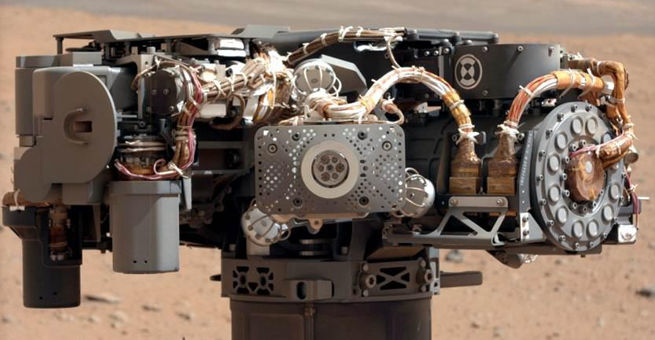
\includegraphics[width=0.475\textwidth]{curiosity_apxs.jpg}
	\tiny{Credit: NASA/JPL-Caltech/MSSS}
\end{center}

The software controlling Curiosity's arm is an improvement over the previous rovers.
This lets the arm get closer to samples on the ground while keeping the instruments safe.
In addition, the amount of radioactive material used in the source has been doubled, which increases the intensity of the ray.
Since the instruments have to operate at low temperatures, Curiosity's APXS has also been equipped with an electrical solid state cooler which lets it function during the Martian daytime.
Spirit and Opportunity could only use their APXS during night on Mars.

Most of the minerals examined contains elements like sodium, magnesium, aluminum, silicon, calcium, iron and sulfur.
APXS can also detect traces of important elements that take part in different salts: sulfur, chlorine and bromide.
These trace elements can be signs of former interactions with water.

After APXS has studied the samples, Curiosity decides if any other tests should be conducted.
The information from APXS is also used to figure out how the stone formations in the area close to the rover could have formed and changed over time.

The radioactive element curium (Cm$^{244}$) is used as a source for the alpha particles.
The element has a half life of 18.1 years, which suits this kind of long term mission.
Even after more than seven years the decrease in activity will be negligible.

The alpha particles emitted are used to excite atoms in the samples, which responds by emitting X-rays afterwards.
These X-rays will be emitted in all directions and the ones coming back towards Curiosity's robot arm can be used in spectroscopy.

Throughout history the different APXS-instruments on the rovers have given us a lot of important data.
Therefore it was brought yet again on Curiosity, and therefore research is still continuing to improve the technique and refine how we will search for water and traces of it in the future \cite{NASA-rover}.

\subsection{Dynamic Albedo of Neutrons (DAN)}
\initial{T}he Dynamic Albedo of Neutrons is an instrument on Curiosity used for the search of hydrogen in minerals or even in ice beneath the Martian surface.
However, it is unlikely that there is any ice directly beneath the surface of the Gale Crater landing site.
The instrument can detect hydrogen up to $50 cm$ below the surface, by shooting neutrons into the ground and measure how they are scattered.

The instrument is a part of the Russian contribution to Curiosity and a broad collaboration between USA and Russia.

In addition to water, DAN can be used to find suiting places to take samples for the other instruments aboard Curiosity.
The data is also complimentary with the camera images and study of the Martian surface and geology.

DAN works by aiming neutrons with high energy at the ground, and registering their energy after they have bounced back.
The loss in kinetic energy is characteristic for each element, and the amount of time it takes for the neutrons to get back, gives an indication of how much of said element is in the ground.
One of the elements that can be, and has been, detected by DAN is hydrogen.
Already before Curiosity was sent to Mars, this technology was used to find water on the red planet.
Neutrons from the background radiation in the cosmos were used as a source when the Odyssey satellite detected water back in 2002.
The hydrogen was interpreted as water close beneath the Martian surface.

DAN can also use the cosmic background radiation as a source for neutrons, but can also actively shoot neutrons towards the ground for higher resolution and more effective tests.

Hydrogen detected by DAN can be signs of former water that at the time got bound in crystals.
These crystals are called hydrated minerals, and can be left over from a wetter period on Mars.

\subsection{Radiation Assessment Detector (RAD)}
\initial{O}ne essential objective for Curiosity's mission is to study the conditions for future human journeys to Mars, of which radiation is feared to be a considerable constraint.
Curiosity carries its Radiation Assessment Detector (RAD) in order to map what kinds of radiation there are and what the levels are.
RAD points upwards in a 65 degree field-of-view to detect radiation from outer space, both particle radiation and electromagnetic waves.
In application where the purpose is to protect humans from radiation, what is also interesting is how much of the radiation that is ionizing.
Such radiation has enough energy to destroy chemical bonds, for example DNA molecules, events that in repeated occasions can lead to cancer.
RAD can for instance distinguish between such ionizing radiation and harmless radiation.
RAD has in fact been in use during the journey to Mars as well, on which a human would also have been exposed to the radiation. \cite{RAD}

\end{multicols}

\noindent\makebox[\linewidth]{\rule{\textwidth}{0.4pt}}

\section{The Red Planet and the rover}

\begin{multicols}{2}

\initial{B}eing equipped with instruments and protection to tackle the Martian environment, Curiosity was ready to start its mission.
Although almost all the technological barriers had been broken, one of the most important was still standing.
NASA had to get the rover to Mars.
Other rovers have already made the travel, but this time it was a little bit different.

On November 26th 2011, Curiosity left Earth with a one way ticket away from home.
More than eight months later, on August 6th 2012, it arrived the vicinity of Mars.
The only thing between the almost $1000kg$ heavy rover and its final destination was the atmosphere of Mars.
This would be the final major challenge Curiosity had to face!

\end{multicols}

%------------------------------------------------

\begin{tcolorbox}[colback=red!5,colframe=DarkRed!40!black,title=Entry, Decent and Landing (EDL)]
Because of Curiosity’s large weight and size, it could not utilize landing procedures used for earlier rovers.
The new landing method is as unique as it is complicated.
The EDL-phase is therefore a spectacle popularly known as seven minutes of terror (referring to the time it takes after touching the atmosphere until it lands) \cite{CNN_7minterror}. 

The EDL sequence breaks down into four parts; guided entry, parachute descent, powered descent and the sky crane \cite{NASALanding}.

{\centering
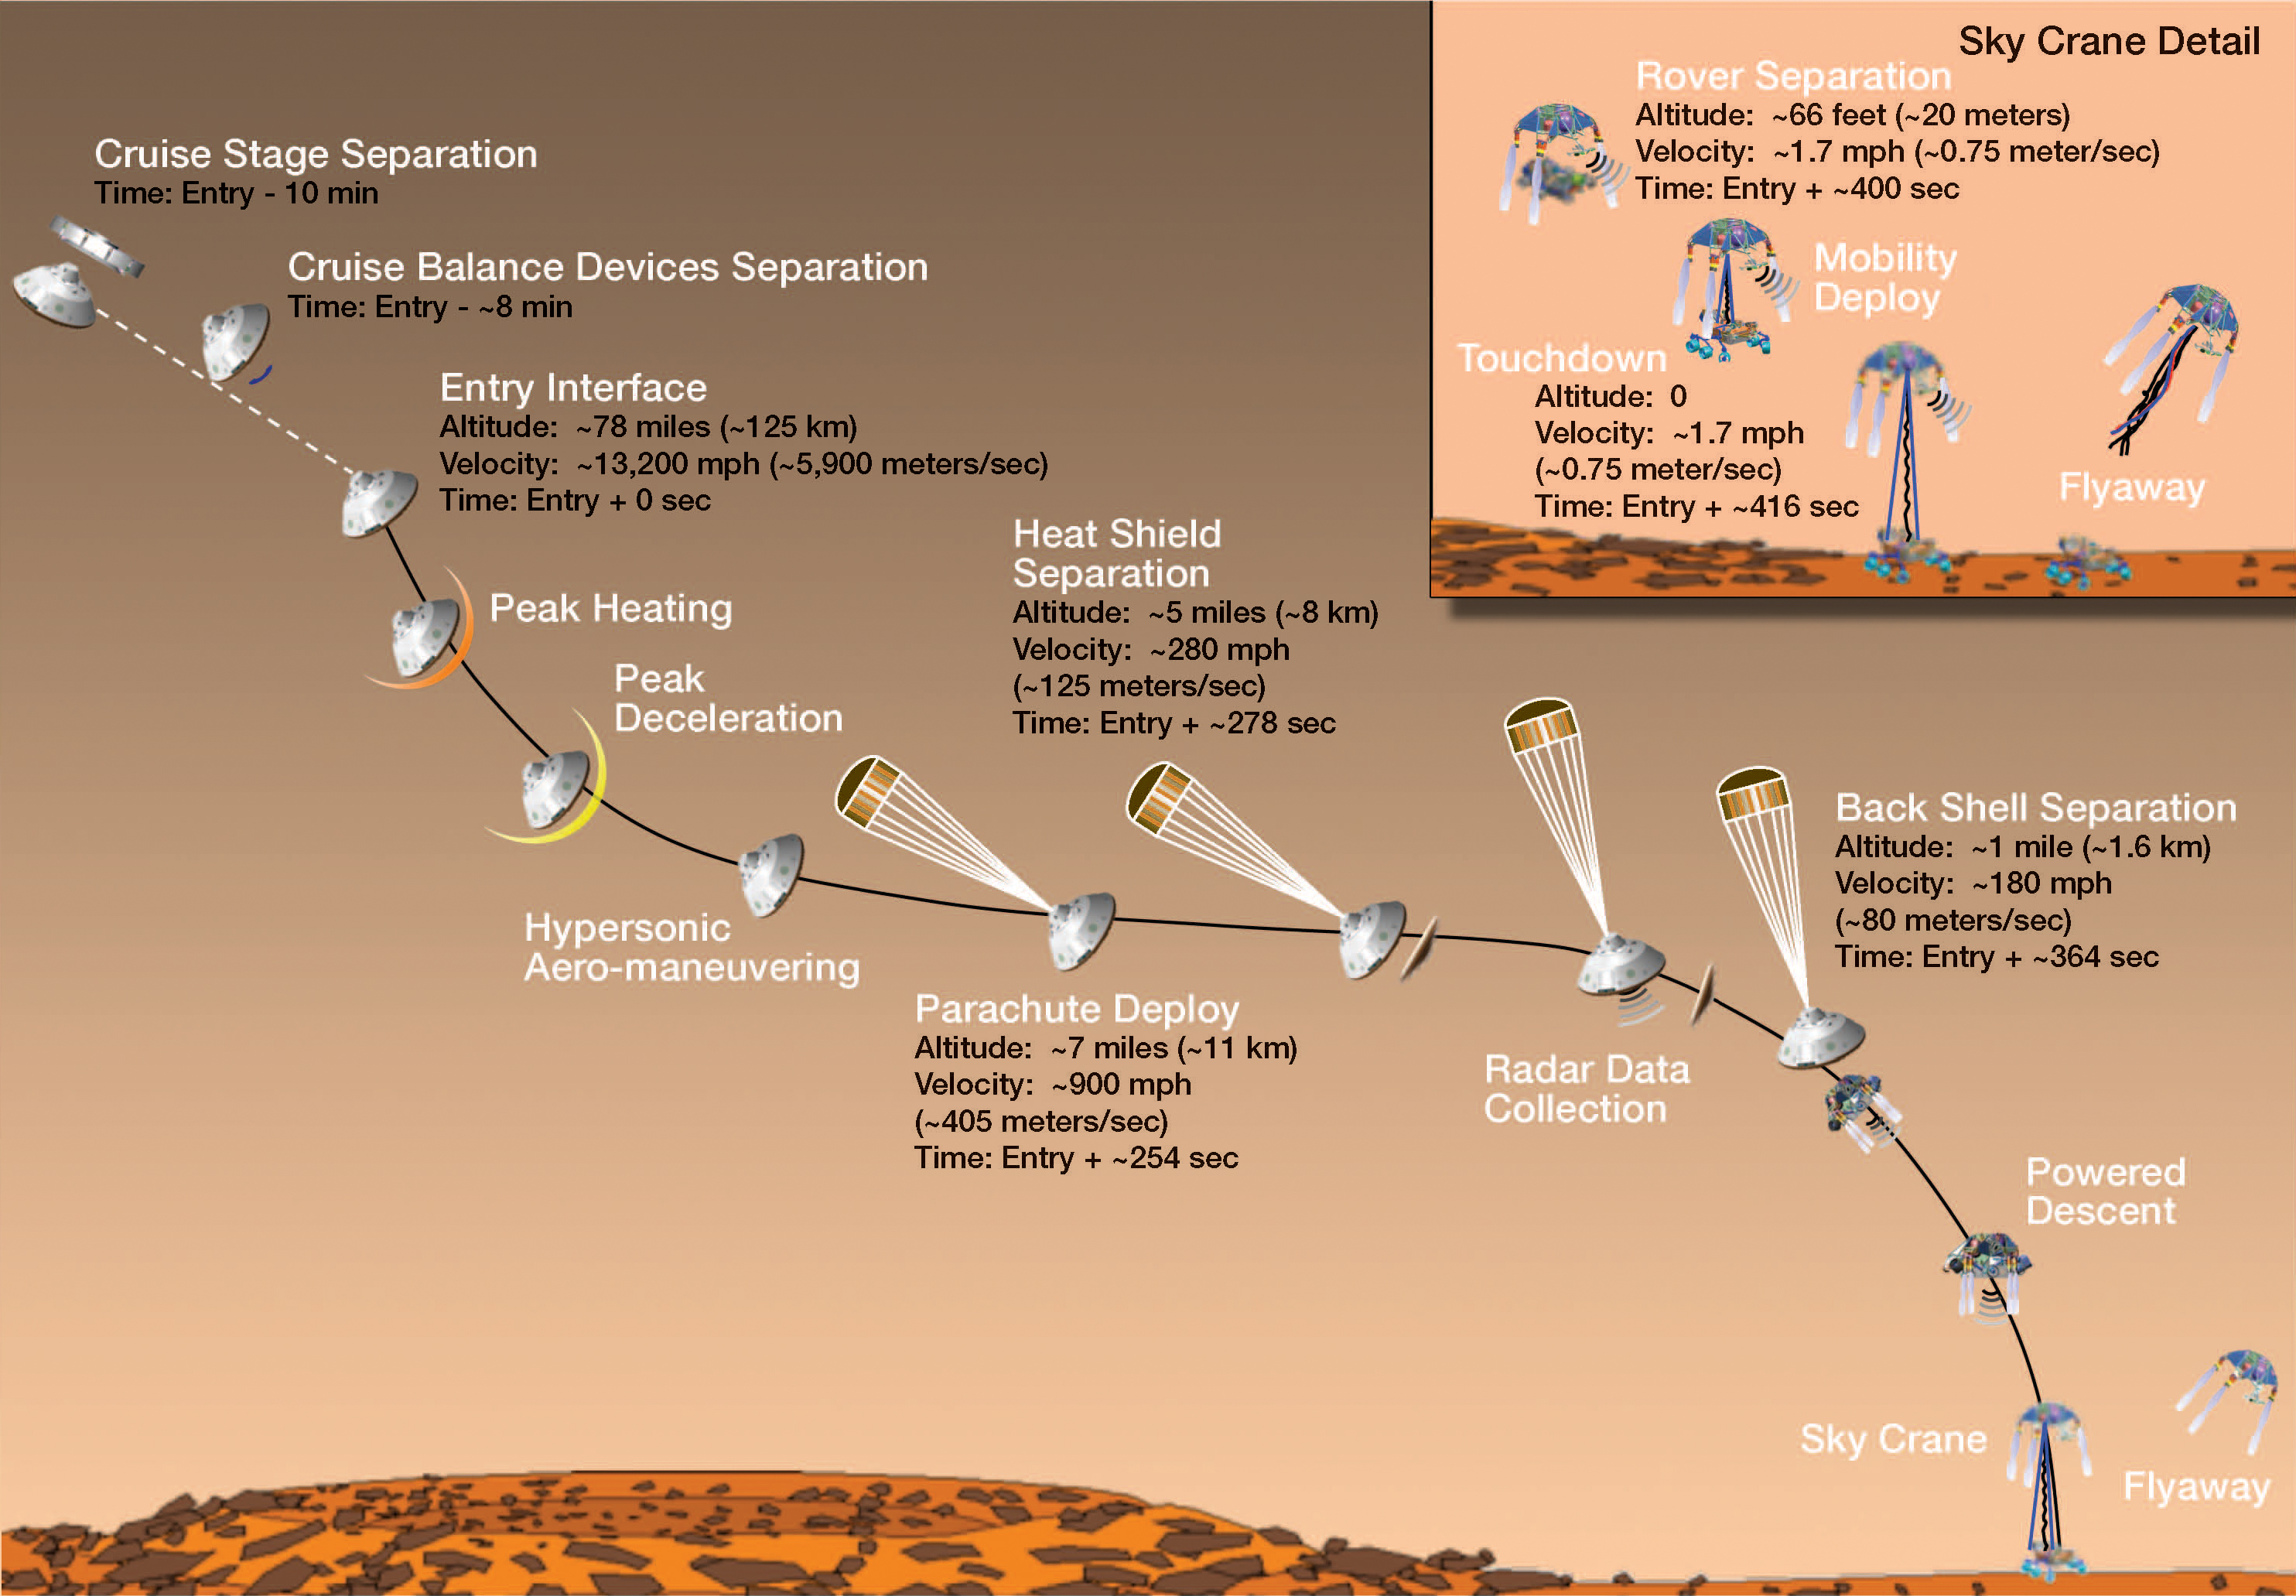
\includegraphics[width=\textwidth]{Curiosity_landing.jpg}
\par}

\textbf{Guided entry}
The spacecraft blasts into the Martian atmosphere at a whopping $21,240km/h$ crating so much aerodynamic drag the heat shield glows at $2,100\degree C$ \cite{NASA_youtube}.
The heat shield only manages to slow the spacecraft to a speed of $1,620km/h$ (because of the thin atmosphere) in which time the deceleration has created a maximum force equal to $16G$s \cite{HistoricLanding} \cite{NASALanding}.

\textbf{Parachute descent}
At this point, the largest and strongest supersonic parachute ever constructed for an extraterrestrial flight deploys. Capable of generating $24,500kg$ of drag force the spacecraft decelerate violently to a speed of $280km/h$ \cite{Parachute} \cite{NASALanding}.
Still way too fast for a landing there is only one solution; cut the rover loose.

\textbf{Powered descent}
The rover now in free fall, accelerates towards the surface at a rate of $3.7m/s^{2}$, fires eight rocket thrusters and reduces the speed to $14.5km/h$ while aiming for the landing site \cite{HistoricLanding} \cite{NASALanding}. 

\textbf{Sky Crane}
At an altitude of $27m$, the rover is detached from the descent stage and slowly lowered to the ground.
The descent speed is reduced to $2.7km/h$ and kept constant.
Then finally, on Aug. 5 2012, after a $5.6 million km$ \cite{CNNCuriosity} journey the rover touches down and pyrotechnically detaches itself from the descent stage.
The decent stage preforms a flyaway-maneuver crash-landing $150m$ away \cite{HistoricLanding} \cite{NASALanding}. 

7 minutes of terror completed.
\end{tcolorbox}

{(!!!no latex formatting yet!!!)

Mars: 10 facts about the red planet

Location: Mars is the 4th planet from the Sun and is the second smallest.
Size: About half the diameter of the Earth. A 100kg person would weight 38kg on Mars.
Magnetism: It has no spinning iron core and thus no planet-wide magnetic field.
Orbit: The distance from the Sun due to the elliptical orbit varies significantly more than on Earth.
Time: A year lasts for 687 Earth days. Martian day = sol = 24 hours, 39 minutes and 35 seconds.
Atmosphere: The atmosphere mainly consists of carbon dioxide (95,3%), nitrogen (2,7%) and argon (1,6%). Atmosphere on Earth has 100 times the pressure than on Mars.
Climate: Temperatures varies from -128C to 27C with an average of -53C.
Geography: Olympus Mons, the tallest known mountain, is 26km, which is approximately 3 times as tall as Mount Everest. Valles Marineris is the solar systems' largest and deepest known system of valleys.
Moons: Mars has two moons: Deimos and Phobos.
Surface: The surface has minerals containing silicon, oxygen and metals. Its red colour comes from iron oxide.

\section{Plans for the near future}

\begin{multicols}{2}

Mars is by far the most investigated planet besides from Earth.
There are spent enormous amounts of money on the search for water and signs of biosignatures, but is Mars the best choice to search for life?
Are there other candidates suitable for supporting life? 
As mentioned on numerous occasions liquid water is a key factor when we are talking about life. 
The Goldilock zone describes the region in space where a planet has just the right distance from its home star resulting in neither too hot nor too cold temperatures for liquid water to exist \cite{FPlan26}. 
Our solar system turns out to be quite an interesting place where liquid water is found on numerous unexpected locations. 
Dr. McKay, who studies the possibility of life in alien worlds, states: "after spending so many years going after Mars, which is so dry and so bereft of organics and so just plain dead, it is wonderful to go to the outer solar system and find water, water everywhere!" \cite{FPlan09}.
Where is this water we are talking about, and how are we going to search for life there?
 
\subsection*{Mars}

First, we look at Mars. 
As mentioned Mars is by far the most explored planet besides Earth. 
How are we going to continue the exploration in the future?
President Barack Obama have tasked NASA with the goal of getting astronauts to Mars, or in Mars' orbit by the mid-2030s. 
This, as well as the Mars One-program, aiming to establish a permanent human settlement on Mars \cite{FPlan12}, have shaped the exploration strategy. 
So far, the only question has been "are we alone?" 
The new strategy poses another, more critical question; "is it safe for humans?" \cite{FPlan01}.

\subsubsection*{Mars 2020 rover}

The Mars 2020 rover mission is NASAs next contribution to the exploration of the red planet. 
Building on Curiositys great landing system the mission will launch in 2020 taking advantage of the favorable orbital positions of Mars and Earth \cite{FPlan14}. 

\begin{center}
	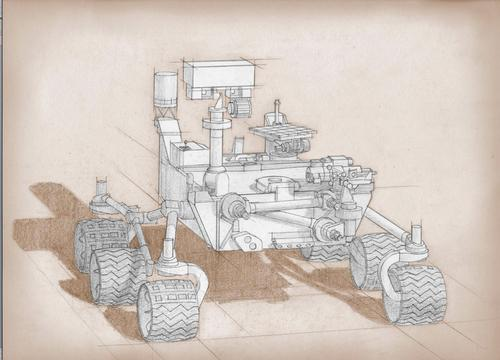
\includegraphics[width=0.45\textwidth]{2020_Rover_Sketch.jpg}
\end{center}

The 2020 rovers’ mission have four main goals \cite{FPlan13}.

\begin{enumerate}
	\item \textbf{Determine whether life ever existed on Mars}
The rover is going to look for sign of biosignatures preserved in rock samples formed in the ancient Martian environment.
This will be the first rover to seek for actual signs of past microbial life.
Earlier missions has focused on establishing if Mars ever had habitable conditions.
	\item \textbf{Characterize the Climate of Mars}
The rover will look for signs that Mars might have provided a habitable environment for microbial life in the past.
	\item \textbf{Characterize the Geology of Mars}
Studying the processes that created and modified the Martian surface by examining the rock record.
Every layer of rock in the Martian crust reveals a record of the environment in which it was formed.
	\item \textbf{Prepare for Human Exploration}
This goal relates to the US’s national space policy of getting an astronaut to Mars by the mid-2030s.
The rover will demonstrate key technologies for using natural resources in the Martian environment to fuel and life support.
\end{enumerate}

It will also measure environmental conditions that might be hazardous for future human travelers.

\end{multicols}

{%kilde: http://www.telegraph.co.uk/news/science/space/10200818/Dangers-of-a-manned-mission-to-Mars.html

\begin{tcolorbox}[colback=green!5,colframe=green!40!black,title=5 dangers for humans to overcome at Mars]
\textbf{Atmosphere:} It is impossible to breath in, due to its low density, as well as its high complex of carbon dioxide.

\textbf{Radiation:} There is constant background radiation on Mars, but there is also a much stronger direct radiation from the Sun. With no significant protection from the Martian atmosphere or a planet wide magnetic field, radiation can reach intensities enough to ionise atoms and thus split chemical compounds, making the environment though to any living creature we know of.

\textbf{Climate:} Liquid water is not known to occur on Mars, however the poles have permafrost. The warmest climate, and thus the most friendly to humans, on Mars is to be found around its equator.

\textbf{Meteorites:} Mars is located near an asteroid belt, and with weak protection from the atmosphere, the Martian surface gives a clue on how great consequences these impacts may cause.

\textbf{Health:} Living in low gravity causes the human body to slowly fall apart. This is crucial when travelling to Mars, but could also be significant at the Martian surface. It is also expected that isolation so far from home could affect the traveller's mental health.
\end{tcolorbox}}

\begin{multicols}{2}

\subsubsection*{ExoMars}

ESA (the European Space Agency) considers the question 'did life ever exist on Mars?' as one of the most important scientific questions of our time.
To address this the ExoMars-program was established.
The goal of the mission is to investigate the Martian environment and to demonstrate new technologies paving way for a future Mars sample return mission in the 2020’s \cite{FPlan02}. 
The ExoMars-program are divided into two missions.
The first consisting of an orbiter (Trace Gas Orbiter) plus an entry, descent and landing demonstrator module (launches in January 2016).
The second featuring a rover dated to launch in 2018.
 
\begin{center}
	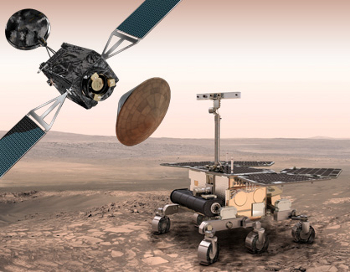
\includegraphics[width=0.45\textwidth]{ExoMars.jpg}
\end{center}

The ExoMars Trace Gas Orbiters main objective is to search for evidence of gases of possible biological importance in the Martian atmosphere, such as methane and its degradation products.
It will also serve as a data relay asset for the 2018 rover mission.
The ExoMars Entry, Descent and Landing Demonstrator Module’s (EDM) objective is to provide ESA with the necessary technology for a controlled landing on the surface of Mars.
The EDM is not going to survive on Mars.
After a short time the batteries runs out and the module shuts down.
Scientific recordings are limited; however, some sensors will be included to preform limited, but useful measurements.
After a nine-month journey, the ExoMars rover hopefully lands unharmed on the surface of Mars.
The rover’s main objective is to travel across the Martian terrain and search for signs of life.
ExoMars will be the first mission to combine the ability to move across the surface and to examine Mars at depth.
With a drill capable of reaching a depth of two meters, it collects samples and analyze them with next-generation instruments.
The goal is to identify organic material from the planets early history.

\subsubsection*{Sample return mission}

A sample return mission (MSR) would collect a sample of ruck and dust on the surface of Mars to return to Earth.
This would be a giant leap in the exploration of Mars because it frees us from the time, budged and space constraints of spacecraft sensors.
All of Earth’s laboratories could potentially study the samples \cite{EarthAnalysis}.
 
\begin{center}
	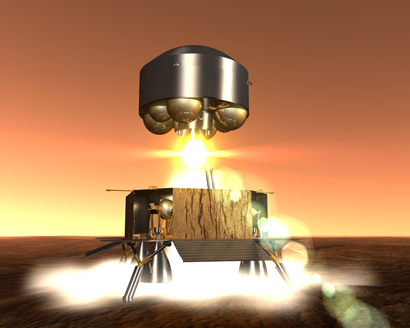
\includegraphics[width=0.45\textwidth]{Sample_return_concept.jpg}
\end{center}

Initially the ExoMars program was a joint project between NASA and ESA with the final goal of a sample return in the mid-2020s \cite{FPlan15}.
Under the FY2013 budget President Barack Obama released in early February 2012, NASA had to withdraw from the joint missions because of budget cuts \cite{FPlan16}.
ESA continues the program without NASA, but there is still no fixed launch date for a sample return mission.
Russia and China are also working on concepts for a sample return mission without any specific timeframes \cite{RussiaPlan} \cite{ChinaPlan}.

\subsection*{Europa}

\begin{tcolorbox}[colback=red!5,colframe=DarkRed!40!black,title=Europa \cite{Europa}]

{\centering
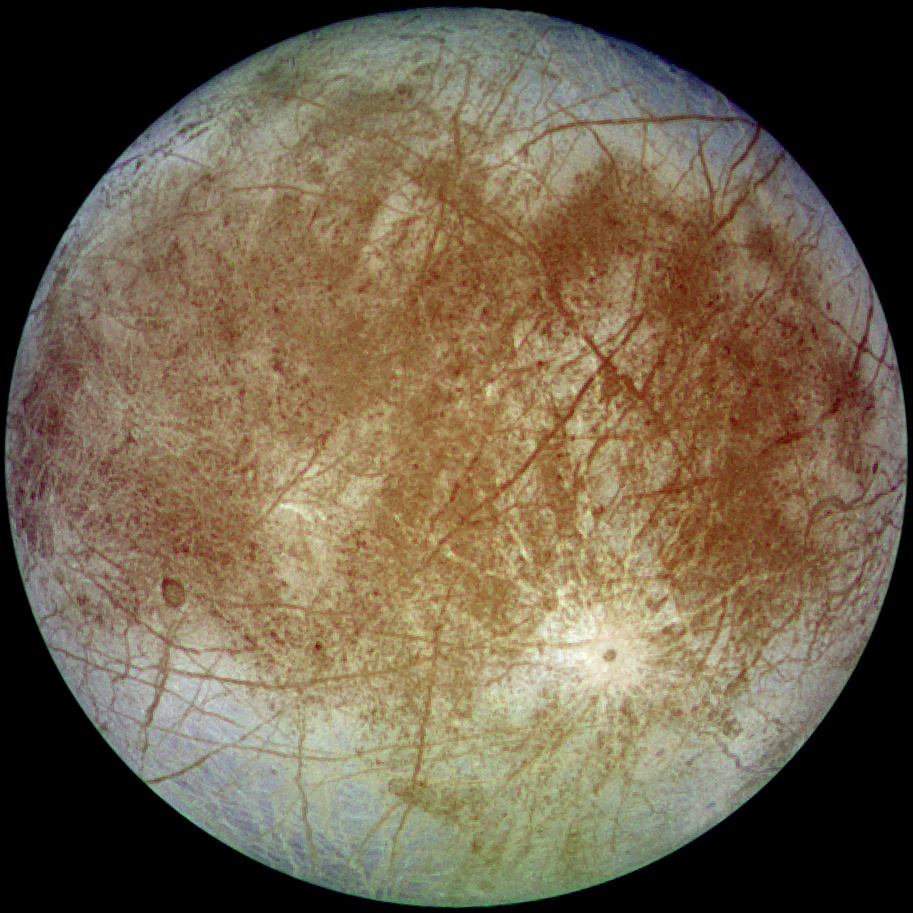
\includegraphics[width=\textwidth]{Europa_moon.jpg}
\par}

\textbf{Satellite of:} Jupiter

\textbf{Diameter:} $3120km$ ($0.245$ Earths)

\textbf{Mass:} $4.8\cdot 10^{22}kg$ ($0.008$ Earths)

\textbf{Surface temp.:} $-171.15\degree C$

\textbf{Gravity:} $0.13 G$s

\textbf{Surface pressure:} $10^{-12} atm.$
\end{tcolorbox}

% solarsytem.nasa.gov/planets/profile.cmf?Object=Jup_Europa&Display=Facts
% Name Europa: Facts & Figures
% Date 22.04.15
 
Europa is one of Jupiter's 64 moons.
With a diameter of 3121.6 km, it is the sixth largest moon in the solar system and would be classified as a dwarf-planet (just like Pluto) if it orbited the sun.
With a mean surface temperature of -171.15\degree C, this is indeed a very cold world.
Ice covers the entire surface, and the atmosphere is weary thin, about 10-12 times earth's atmosphere.
At first glance, it does not look habitable, but scientists actually believe this to be one of the most likely places to find life in our solar system.
Because of tidal flexing, a process caused by Jupiter’s strong gravity and Europa’s slightly eccentric orbit as well as orbital resonance with the other moons, it generates heat melting the ice from inside.
Scientists believe the moon to have a 100 km thick layer of liquid water under 30 km of ice \cite{FPlan03} \cite{FPlan24}.
 
In 1977, scientists discovered life independent of sunlight concentrated around underwater volcanic features known as black smokers.
In addition, it was recently discovered bacterial life in a Lake Whillans 800 meters below the Antarctic icecap \cite{FPlan04}. This strengthen the theory of life on Europa.
There are currently three different projects in work to look for life on Europa: Juice, Europa Clipper and Valkyrie \cite{FPlan24}.
Juice is an ESA engaged mission featuring an orbiter planned to launch in 2022.
The orbiter is going to visit the Jupiter moons Europa, Callisto and Ganymedes.
It is only going to pass Europa twice in which time it will measure the thickness of the ice as well as mapping the surface in detail.
The wide range of instruments will also reveal the moons internal structure and chemical environment \cite{FPlan24}.
NASA is also going to send an orbiter planned to launch in 2025.
The spacecraft is going to pass Europa 45 times while orbiting Jupiter.
With a variety of instruments shall examine the same factors that Juice \cite{FPlan24}.
Most exiting is the NASA engaged mission Valkyrie.
Valkyrie is an autonomous robot that will drill through the thick ice and explore the ocean underneath it.
The robot consists of a long cigar formed tube melting its way through the ice powered by a 5000-watt laser carried through a fibre optic wire from a nuclear power source on the surface.
Tests conducted in Alaska have shown that Valkyrie is able to move at a rate of almost one meter per hour \cite{FPlan24} \cite{FPlan25}.

\subsection*{Titan}

\begin{tcolorbox}[colback=red!5,colframe=DarkRed!40!black,title=Titan \cite{Titan}]

{\centering
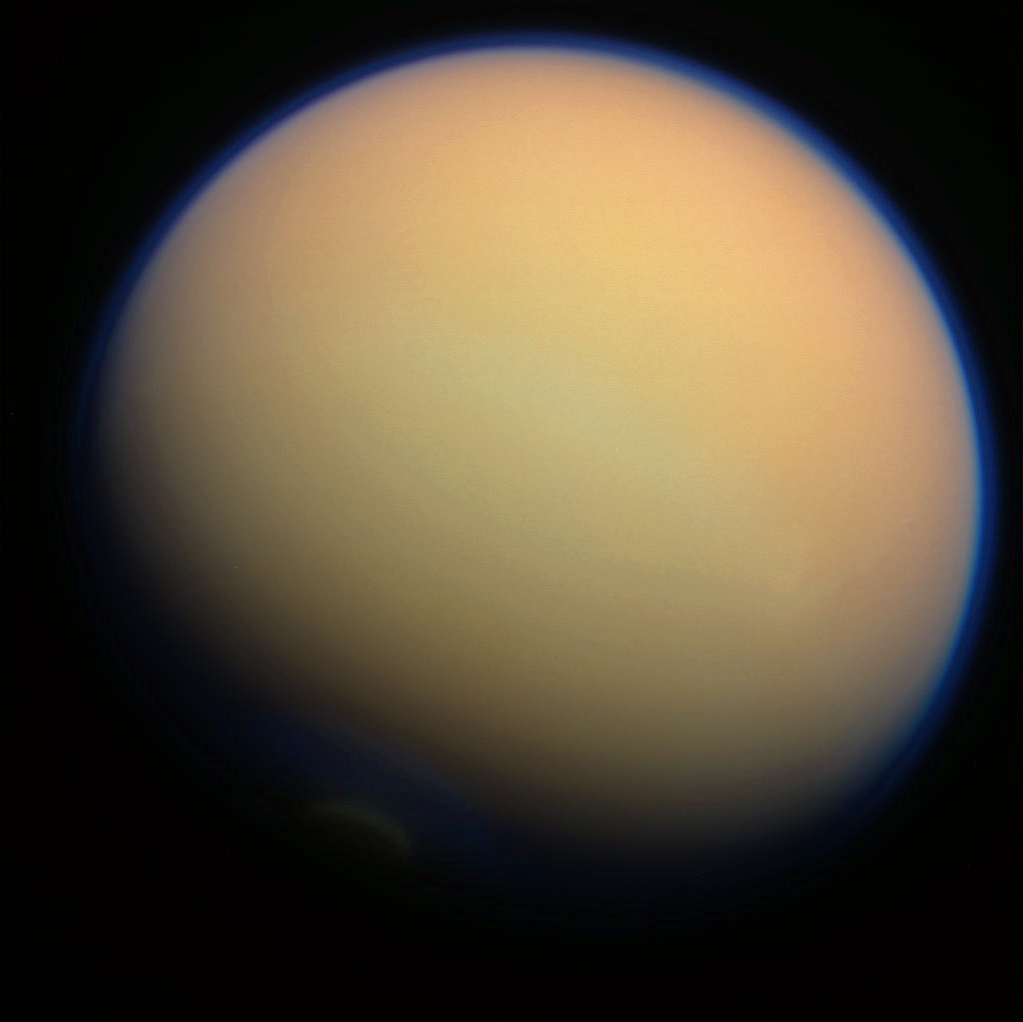
\includegraphics[width=\textwidth]{Titan_moon.jpg}
\par}

\textbf{Satellite of:} Saturn

\textbf{Mean diameter:} $5,150km$ ($0.404$ Earths)

\textbf{Mass:} $1.35\cdot 10^{23}kg$ ($0.023$ Earths)

\textbf{Surface temp.:} $-179.5\degree C$

\textbf{Gravity:} $0.14 G$s

\textbf{Surface pressure:} $1.45 atm.$
\end{tcolorbox}

% http://solarsystem.nasa.gov/planets/profile.cfm?Object=Sat_Titan&Display=Facts
% Name Titan: Facts & Figures
% Date 22.04.15
 
Titan, one of Saturn's 62 moons, have also caught scientists' attention.
With a diameter of 5150 km, it is the second largest moon in the solar system, and just like Europa, Titan is very cold.
Receiving only 1\% of sunlight compared to earth the surface temperature is about -180\degree C.
Titan is actually the only known moon with a significant atmosphere, and despite the lower gravity, it has a larger atmospheric pressure than earth (about 1.45 atm.).
What intrigues scientists is the environmental similarities with the theoretical primordial Earth.
Titan is thought to be a prebiotic environment rich on complex organic chemistry \cite{RichOrganics}. On the other hand, the lack of liquid water have led some scientists to consider life as unlikely.
However, Titan is rich on other compounds like for hydrocarbons a.m.
These could replace water as a solvent (read more about this hypothesis later).
Resent years it is proposed several interesting conceptual missions for sending a space probe to Titan. Unfortunately, all of these have yet to be funded.
The Titan Saturn System Mission (TSSM) was created by merging ESA’s Titan and Enceladus Mission (TandEM) with NASA’s Titan Explorer in January 2009 \cite{FPlan10}.
TSSM was an ambitious mission featuring a hot air balloon flying in Titans thick atmosphere.
Carried by the winds it could circle the moon in only six months and would have managed two circumnavigation in its design one-year lifetime.
Early February 2009 ESA and NASA announced that a Europa-Jupiter mission had priority ahead of TSSM \cite{FPlan07}.
It has also been proposed two different concepts featuring a lake-lander, TiME (Titan Mare Explorer) and TALISE (Titian Lake In-situ Sampling Propelled Explorer).
Splashing into a lake on the northern hemisphere, it would float in the cold methane liquids \cite{TiME} \cite{TALISE}.
In addition, a mission consisting of an unmanned drone (AVIATR) was proposed in early 2012, but NASA did not approve the requested \$ 715 million for the project \cite{AVIATR}.

\subsection*{Enceladus}

\begin{tcolorbox}[colback=red!5,colframe=DarkRed!40!black,title=Enceladus]

{\centering
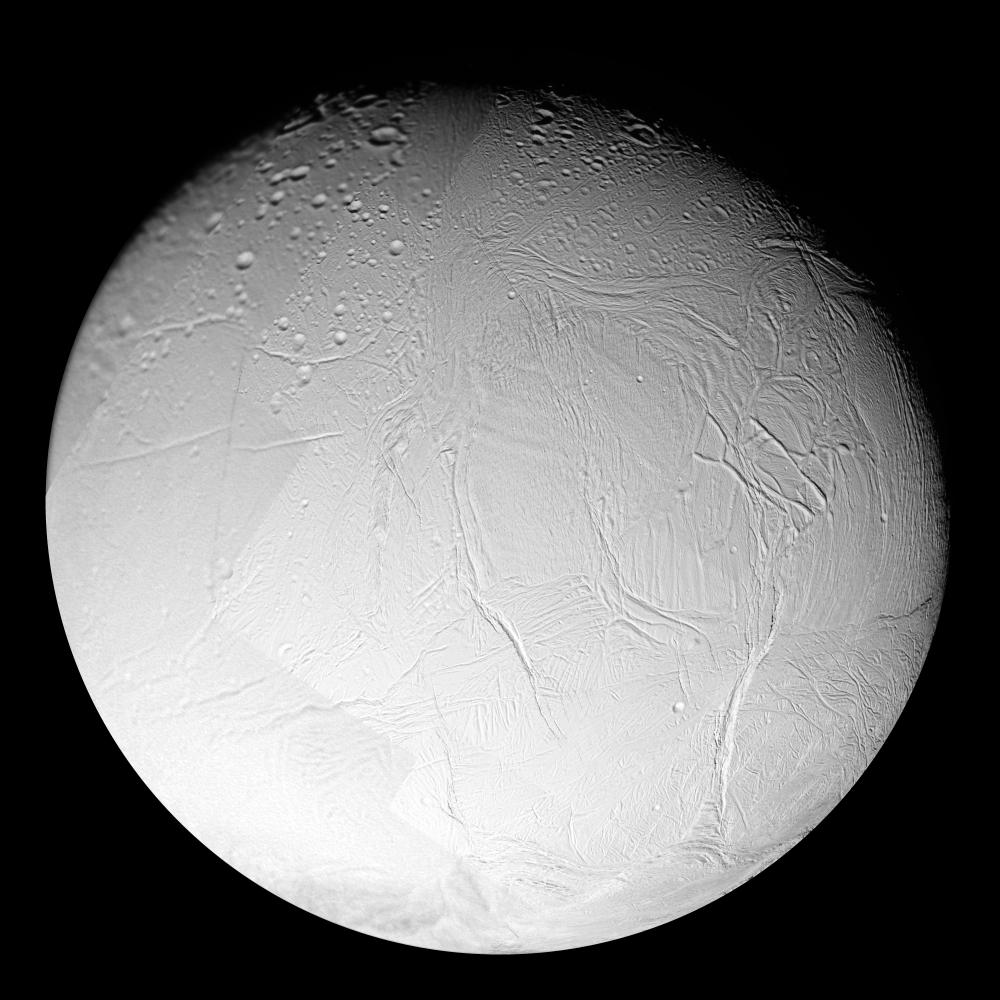
\includegraphics[width=\textwidth]{Enceladus_moon.jpg}
\par}

\textbf{Satellite of:} Saturn

\textbf{Mean diametre:} &504km& (&0.04& Earths)

\textbf{Mass:} $1.08 \cdot 10^{20}kg$ (&1.8 \cdot 10^{-5}& Earths)

\textbf{Surface temp.:} &-178 \degree C&

\textbf{Gravity:} &0.012 G&s

\textbf{Surface pressure:} &---&
\end{tcolorbox}

% solarsystem.nasa.gov/planets/profile.cmf?Object=Sat_Enceladus&Display=Facts
% Enceladus: Facts & Figures
% Date 22.04.15
 
Enceladus, another of Saturn’s 62 moons turns out to be more interesting than previously assumed.
With a radius of only 500 km, it is much smaller than Titan, but still the sixth largest orbiting Saturn.
Just like Europa and Titan, Enceladus is very cold.
With a mean temperature at approximately -198\degree C, ice covers the entire surface.
Before the Cassini spacecraft started multiple close flybys in 2005 Enceladus was thought to have liquid water under the ice.
When the flybys started, it discovered cryovolcanoes near the South Pole shooting geyser-like jets with velocities up to 2189 km/h (equivalent to 1.8 times Mach 1 under normal conditions on Earth) into space.
Measurements revealed that the cryovolcanoes consisted of water vapor, other volatiles, and solid material like crystals and ice particles \cite{Enceladus1}.
Scientists’ also reports evidence of hydrothermal vents.
If this turns out to be correct, Enceladus would be the only known place, besides from earth, with such chemical reactions between rock and heated water \cite{FPlan09}.
The Cassini missions have provided evidence of several nutrients and organic molecules.
The combination of an internal salty ocean with hydrothermal vents and simple organic compounds makes this a potentially habitable environment for microbial extraterrestrial life.
The Titan and Enceladus Mission (TandEM) was, before merging with NASAs Titan Explorer (crating Titan Saturn System Mission, TSSM), a mission to study the Saturnian moons Titan and Enceladus, with special emphasis on Enceladus \cite{FPlan11}.
TSSM mainly focused on Titan but the missions’ orbiter would do a minimum of seven close flybys analyzing the cryovolcanic plumes.
There are unfortunately no current plans to send a spacecraft to Enceladus, or Titan for that matter.
Both NASA and ESA seems to focus on Europa first.

\subsection*{Other possible goals}

Both Ganymede and Callisto (moons of Jupiter) seems to have hidden water under the surface \cite{FPlan09}.
Every place in the universe harboring liquid water is considered interesting and the moons could potentially support life, though less likely than Europa, Titan and Enceladus.
Scientists has also pointed out Venus as a potential place to habitat life.
At first glance, it might not look habitable.
With a mean surface temperature of 462\degree C (hot enough to melt led) and an atmospheric pressure 90 times that on Earth even the spacecraft that landed on Venus was crushed and melted within a couple of hours \cite{FPlan17} \cite{FPlan18}.
However, reputable scientists like Carl Sagan, David Grinspoon, Geoffrey A. Landis and Dirk Schulze-Makuch suggest a hypothesis of microbes existing in cloud layers 50 km above the surface \cite{LifeVenus}.
Temperatures here would be refreshingly tolerable.
Atmospheric sulfur dioxide and carbon monoxide might serve as food for the floating microbes \cite{FPlan20}.

Ceres is the largest known object in the asteroid belt, but still the smallest known dwarf planet \cite{FPlan21}.
On March 6, 2013, infrared readings from the Herschel space observatory confirmed water vapor rising from the surface. It is suggested that Ceres possess subsurface liquid water, and perhaps traces of life \cite{FPlan22}.
The Dawn mission, led by NASA, is the only spacecraft that has visited Ceres \cite{FPlan23}.
It has neither confirmed nor disproved the theory of liquid water.


% Super ball bot?

% How will we search?

%------------------------------------------------

\end{multicols} \noindent\makebox[\linewidth]{\rule{\textwidth}{0.4pt}}

\section{Other forms of life}

\begin{multicols}{2}

\initial{S}o far, our pursuit for extraterrestrial life has been based on our knowledge from Earth.
As we already know, all known life on our planet is based on carbon compounds and water as a solvent \cite{OForm2}.
But as William Brains stated concerning these molecules in 2004: "this is not an inevitable conclusion from our knowledge of chemistry" \cite{OForm1}.
So if we open our minds, what could then exist out there?
Moreover, where could it exist?
And what could potentially replace these substances?

\subsection{Non-carbon based life}

\initial{F}irst, let us focus on carbon. Several prominent scientists are concerned that we might be blinded by our familiarity with carbon and Earth-like conditions.
It is not beyond the realm of feasibility that our first encounter with extraterrestrial life will not be a solely carbon-based \cite{OForm3}.
Several compounds might do the same trick.

Silicon is the most promising element to replace carbon as a basis for an alternative biochemical system. 
Located directly beneath carbon on the periodic table, silicon has similar chemical properties as carbon \cite{OForm4}.
Silicon has the same number of electrons in its outer shell, meaning it can form four bonds just like carbon.
Another shared property is that silicon can bond to itself making Si-Si bonds and therefore form large enough molecules to carry biological information \cite{OForm5}.
This might sound promising, after all C-C bonds are the basis for complex molecules on Earth \cite{OForm4}.
Another of carbon's vital features is that it can form chemical bonds with many other atoms creating organic functional groups.
The chemical versatility required to conduct the reactions of biological metabolism and propagation is caused by carbons ability to bond with hydrogen, oxygen, nitrogen, phosphorus, sulfur, as well as metals such as iron, magnesium and zinc.
Silicon, in contrast, interacts with only a few other atoms making it monotonous compared with carbon \cite{OForm5}.

Some of the most common carbon molecules on Earth, such as carbon dioxide CO2 and methane CH4 do have silicon derivatives (silicon dioxide SiO\textsubscript{2} and silane SiH\textsubscript{4}).
Although SiO\textsubscript{2} is common on Earth (quartz), it is, in contrast to CO\textsubscript{2} a solid at temperature below 2000\degree C.

So far, we have compared silicon and carbon within the context of earth-like conditions.
This does not have to be the case for other planets.
Can you imagine a silicon-based organism, living in a 3000 degrees atmosphere?
It may sound unlikely, but chemistry able to support life does not have to be within the temperature ranges we find comfortable.
Even here on earth one specie's sweet spot could be another specie's worst nightmare.

Biochemists also speculate whether there are other substances that could replace carbon.
In theory, many elements could work.
Even counter-intuitive elements such as arsenic may be capable of supporting life under the right conditions.
Actually, some marine algae is reported to incorporate arsenic into complex organic molecules \cite{OForm3}.
Chlorine, nitrogen, phosphorus and sulfur are also possible elements to replace carbon.
Sulfur and phosphorus are capable of forming long-chain molecules much like carbon and some bacteria have been discovered to survive on sulfur rather than oxygen \cite{OForm3}.

\subsection{Non-water solvent}

\initial{W}ater is considered a key factor when searching for extraterrestrial life.
Prominent scientists, such as Carl Sagan, believe carbon to be difficult to replace, but that water is less essential \cite{OForm2} \cite{OForm3}.

Ammonia, for example, has many of the same properties as water.
It can dissolve most organics as well as or better than water, and it has the unprecedented ability to dissolve many elemental metals such as sodium, magnesium and aluminum.
Several other elements such as iodine, sulfur, selenium and phosphorus are also somewhat soluble in ammonia with minimal reaction.
All these elements are important in biochemistry capable of supporting life.
The vital solvent for a living organism should be capable to permit acid-base reactions.
By using ammonia as a solvent the acids and bases are quite different than when using water because acidity and basicity are defined relative to the medium in which they are dissolved. Therefore, water and ammonia are not chemically identical but just simply analogous.
However, on the down side, the temperature range in which ammonia stays liquid is rather small compared with water (at one atm.) and the surface tensions are only one third of as much.
The hydrogen bonds that exist between ammonia molecules are also much weaker than those in water \cite{OForm7}.

Ammonia or an ammonia-water mixture has a substantial lower freezing temperature \cite{OForm3}, and this brings us back to Titan, one of Saturn's moons.
Rich on complex organic chemistry but way too cold to hold liquid water it is considered unsuitable to support life.
Considering alternative biochemistry by replacing water with ammonia Titan would be highly capable to support extraterrestrial life.

Stephen Hawking has several exciting ideas about extraterrestrial life.
He imagines lifeforms independent of water as a solvent.
Nitrogen exists as a gas at normal conditions, but at very low temperatures, -196\degree C or lower, it becomes a liquid resembling water \cite{OForm6}.
Does a world exist, far beyond the habitable zone, holding large oceans of liquid nitrogen capable of supporting life?
This idea is as intriguing as it is unlikely.
Nitrogen and water have quite different chemical properties.
However, as Stephen Hawking underlines, with a radically different environment, comes radically different chemical reactions.
Water and carbon might be the very last things capable of supporting life in some extreme planetary conditions \cite{OForm3}.

All of these ideas might sound just a bit too incredible and unlikely, but actually, it has some emphasis. 
Discoveries over the past decades revealed extreme lifeforms thriving at highly unlikely places, such as superheated walls of ocean-volcanic vents and the interior of the planets crust.
The NASA sponsored report recommends that the search for life should be widened to include the possibility of "weird" life.
It concludes: "Nothing would be more tragic in the American exploration of space than to encounter alien life and fail to recognize it" \cite{OForm3}.

If we open up for these possibilities, life seems suddenly able to exist everywhere, just awaiting to be discovered.

\end{multicols} \noindent\makebox[\linewidth]{\rule{\textwidth}{0.4pt}}

%------------------------------------------------

\section*{What is life, \textit{really}?}

\begin{multicols}{2}

\initial{W}e have just examined the specifics of life at micro scale, but could we be missing the forest for the trees?
There are some creative theories that view life on grander scales, and even predictions that a human invention will one day challenge our concept of life.

\subsection{Life in a computer}
\initial{T}he interest in Artificial Intelligence (AI) has risen in recent years, as business corporations see the opportunity to replace human manpower with computers to enable increased workloads.
Development in this field of study has of course lead to some interesting inventions.
In early 2014 Facebook announced that their face recognition software was as accurate as the human brain \cite{facebook}.
This example shows how inventions in AI have a rather practical approach these days, with single purposes, although the holy grail would be to create a more complex software and even with consciousness.
If algorithms like Facebook's were to be simplified, or when their patents are no longer valid, perhaps even more complex algorithms can be formed.

AI is based on human behavior, and is also connected to psychology.
The assumption that humans are the most intelligent beings, gives us the motivation to try to replicate ourselves.
Despite what many people believe, AI does not have to include fancy robotics and machinery, nor does it have to be an android in physical matter.
An agent, which is the smallest unit of AI, senses, reflects and actuates.
The sensors and actuators gives its physical constraints, and the reflection is core of the AI.
There are two levels of AI: weak AI and strong AI.
Weak AI is when an agent acts intelligent, which disables a Turing test to distinguish it from a human.
The Turing test is a test in which a human judge, holding a conversation with another entity, must deem whether or not that entity is human or machine. 
When it comes to an actual intelligent agent, it is a subject to strong AI.
However this is yet to be made.


\paragraph{The ghost in the machine}

In Philip K. Dicks emph{Do Androids Dream of Electric Sheep?}, which was made into the slightly-more-famed movie \emph{Blade Runner}, the protagonist Deckard works as a policeman specializing in catching runaway and criminal androids. In Deckard's world, artificial intelligence has advanced to such a level that telling the difference between a machine and a human being takes expert level knowledge and the application of a variant of the Turing test, a test in which a human judge, holding a conversation with another entity, must deem whether or not that entity is human or machine. 
While Deckard's machines aren't the end-all, be-all of artificial intelligence, they mark the crucial point in coming human history where human beings and machines become indistinguishable to anything but the trained eye. If we can reach a stage where having a conversation with a machine becomes indistinguishable from having a conversation with a regular human being, then can we say that the machine isn't alive? Can something mechanical be infused with a soul? Can something consisting of copper wires and transistors, designed in a lab and built in a factory, be just as living as something made of organic materials? Is it possible that we will \emph{build} life before we discover it?

\paragraph{Architects of our own demise}
The subject of science as a force for destruction is a well-known issue. Engineering has given us the tools to perform miracles, but also the tools to facilitate our own apocalypse. Recently, debates have grown regarding the future dangers of artificial intelligence - at its highest ideal, artificial intelligence will give birth to entities that will seem \emph{god-like} compared to a regular human being. Infinitely higher capacity for information storage and search, instant learning, physical capabilities and endurances so superiour to our own that we will be powerless to stop them \emph{should we make enemies of these machines}. This is the \emph{Terminator} endworld dystopian nightmare, in which human beings are in the process of being exterminated by the superior technology of the machine race. 
AI experts have split opinions on this potential future. Some believe that these future dangers are negligable; we will always have an element of control, or the machines will have no reason to abuse us, and the benefits of such god-like beings in our employ are beyond imagining. There is also a line of belief that says humanity will end itself before this kind of AI becomes global; the very respectable Hugo de Garis presents his theory on \emph{The Artilect War}\cite{artilect}, in which rival factions within the human race will destroy each other before powerful AI is made. The first of these two factions is convinced of the benefits of AI and wishes to continue to build them, whilst the other is so terrified of the machine future that they make war on the first faction. With such names as Stephen Hawking and Elon Musk (whom, in fairness, are not AI experts) speaking out against the development of AI, a careful eye has to be kept on the development of these technologies. 

\subsection{The Gaia theory}
\initial{B}uilding life is one possibility, maybe we don not have to build life ourselves, but we might already be part of a larger living system.
Considering what we now know of the unwitting coordination of the cells in our body, the Gaia theory is intriguing.
Originally concocted by a chemist named James Lovelock\cite{Lovelock} in the 60s, it is about how the very planet we live on can be a single organism consisting of trillions of lifeforms working together unwittingly.
Could it be that we are just cells in the body of the planet Earth?
Are we zooming around the Sun in a single organic spaceship?
Could we, in the future, as our space travel talents grow, encounter living planets as singular entities?

\subsection{Multiverses}
\initial{I}f you put the most vivid part of your brain in action, there are really no limits on how abstract one can make the concept of life.
Why must \textit{life} be restricted to something close to our own size?
Why must \textit{life} be restricted to something that resembles us at all?
We have mentioned the Gaia theory, but why stop there?
The Universe itself could also be considered a living organism, if what some theoretical physicists believe are true.
This is where we introduce the idea of a multiverse.

The idea goes as follows:
What if there is more than one universe?
What if these are all connected to each other in a dimension completely oblivious to us?
What if universes could create new universes?

\begin{center}
	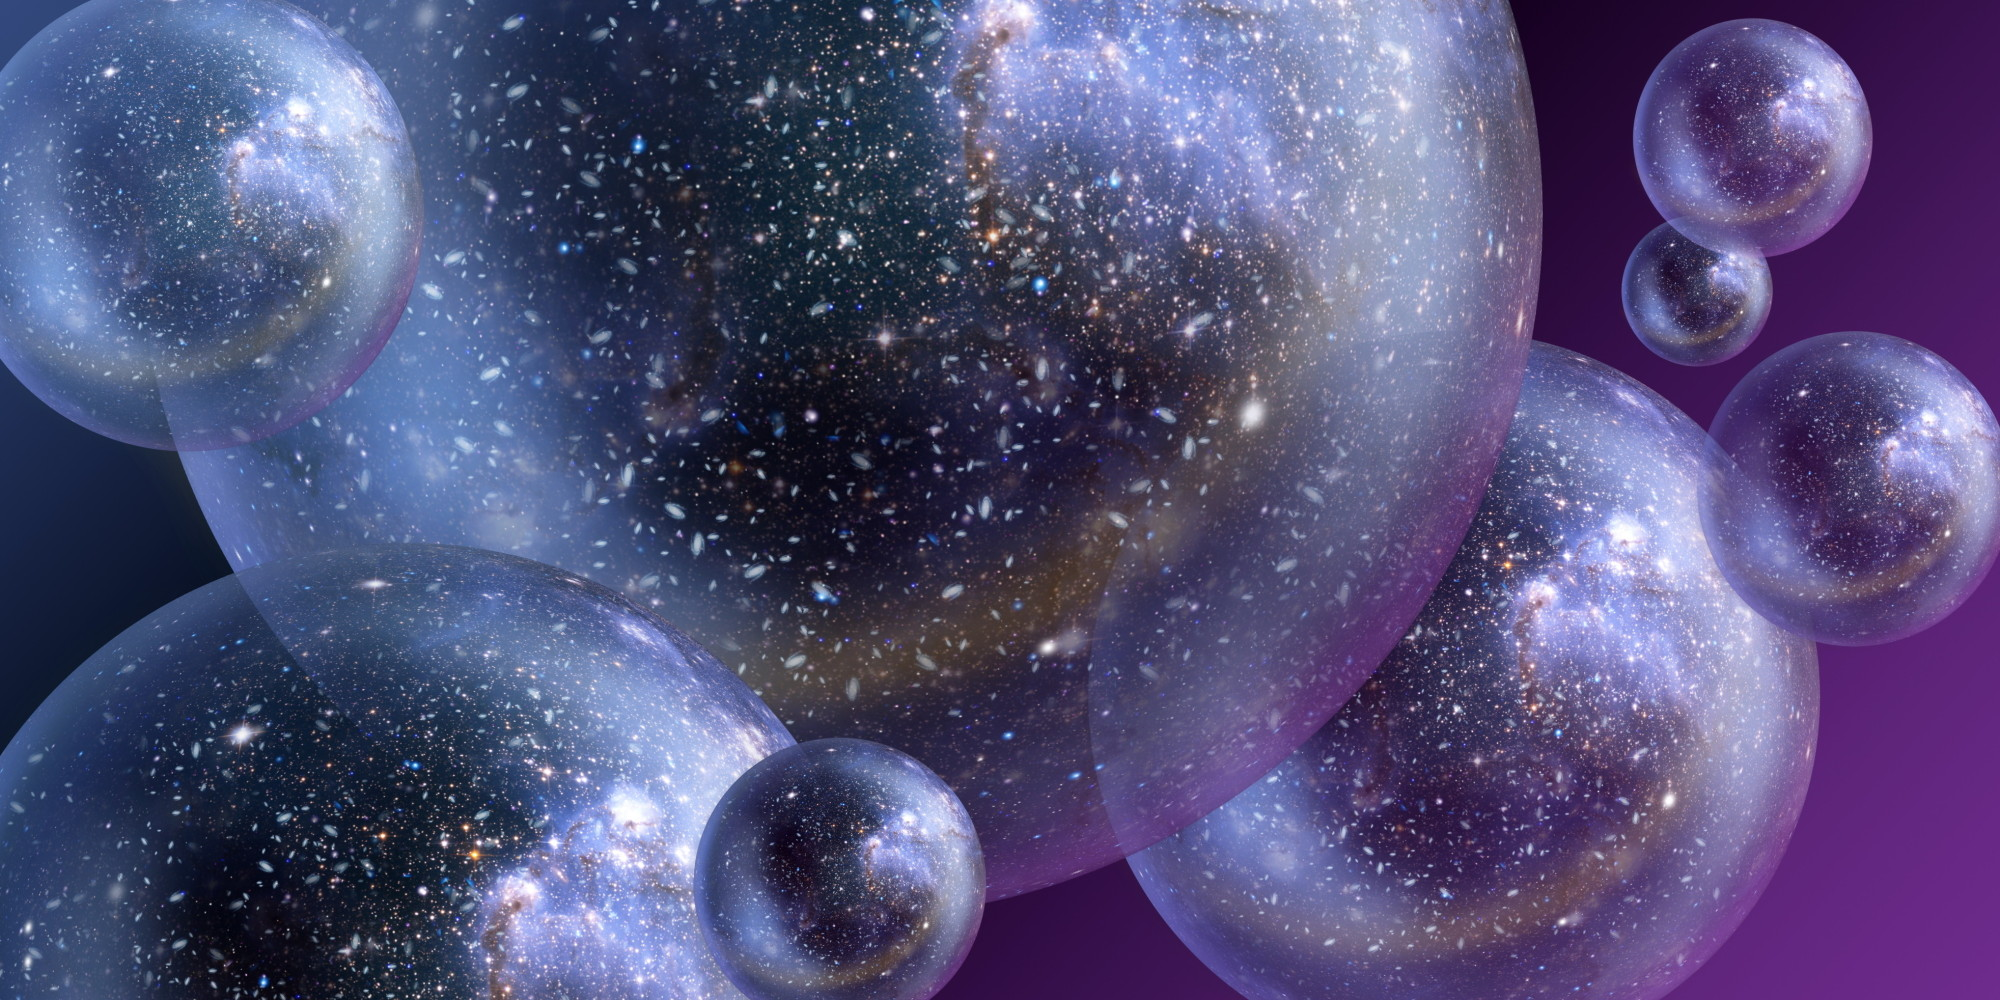
\includegraphics[width=0.47\textwidth]{multiverse.jpg}
\end{center}
%http://i.huffpost.com/gen/2229248/images/o-PARALLEL-UNIVERSES-facebook.jpg

Multiverse has been suggested several times in science fiction, often in context of time travel or alternate universes.
Time travel would for example, split the history into two different universes.
One where the time travel never happened and one where it did.
Alternate universes would often be a thought experiment where you could have been born in a different place and time, but still be \textit{you}.
Could there be a world out there where you are the President of the United States?

There also exists a more scientific, or less fictional, version of this idea.
In short, different universes would have different physical conditions, and all of them would pan out differently one from another.
The beginning of a universe would be something like the Big Bang.
From there it grows and changes, governed by its own physical laws and constants.
In time it may come to a stage where it creates black holes.
Some think this is how a universe might reproduce.
The newly formed universe would have slightly different attributes than its parent.
Some universes may die, some may have physical conditions that keep them in an endless cycle of expanding and retracting.

Universes could undergo birth, growth and death.
They evolve throughout their generations with every infant universe being slightly different from its parent.
Only the ones capable of creating black holes will be \textit{successful}.
How these organisms could feed and move in higher dimensions is even more vivid and far fetched.
After all, this is only an idea.
At least for now.

\initial{H}ow extraordinary to see our journey from the ancient Egyptians' views of the celestial realms to Curiosity landing on the surface of the Red Planet. 
Thanks to our curiosity, the essence of human beings, the world of knowledge is in perpetual progress. 
But \emph{"the more we learn the less we know"} and the philosophical questions around life and our universe remain open.
Where and what is the origin of life? 
We agree on the ingredients needed to form life, but we know little on how these were set together. 
Moreover, is our definition of life too limited? 
Water and carbon are essential for life as we know it today on Earth, but could these be replaced by other substances? 
And if so, is research based on water the right procedure owing to the fact that \emph{"nothing would be more tragic [...] than to encounter alien life and fail to recognize it"} \cite{OForm3}. 
Thanks to the most advanced techniques of communication, laboratory analysis and robot instruments, the rovers based on Mars were able to find and prove earlier presence of water.
It is undeniable that this discovery counts positively on our research of extra-terrestrial life and lead us a step further to answer the most fascinating question: \emph{Are we alone?} 
To answer that question we are forced to search further in our Cosmos, in places like Europa and hopefully new discoveries and new understanding of life await us. 
Even more disturbing and captivating, what if we can seek further in our own definition of life. 
If we fail to find life elsewhere, what about taking the responsibility to produce different life in form of Artificial Intelligence? 
Or what if living things on Earth, like us, are cells part of a bigger organism like the Gaia theory suggests?
Human curiosity has brought us this far, but only future can tell if it will take us \emph{"to the infinity and beyond"} \cite{buzz}.

\end{multicols} \noindent\makebox[\linewidth]{\rule{\textwidth}{0.4pt}}

%----------------------------------------------------------------------------------------
%	REFERENCE LIST
%----------------------------------------------------------------------------------------
\onecolumn
\small{
\input{"Kilder.tex"}
}

%----------------------------------------------------------------------------------------

\end{document}